\documentclass[twoside]{book}

% Packages required by doxygen
\usepackage{fixltx2e}
\usepackage{calc}
\usepackage{doxygen}
\usepackage[export]{adjustbox} % also loads graphicx
\usepackage{graphicx}
\usepackage[utf8]{inputenc}
\usepackage{makeidx}
\usepackage{multicol}
\usepackage{multirow}
\PassOptionsToPackage{warn}{textcomp}
\usepackage{textcomp}
\usepackage[nointegrals]{wasysym}
\usepackage[table]{xcolor}

% Font selection
\usepackage[T1]{fontenc}
\usepackage[scaled=.90]{helvet}
\usepackage{courier}
\usepackage{amssymb}
\usepackage{sectsty}
\renewcommand{\familydefault}{\sfdefault}
\allsectionsfont{%
  \fontseries{bc}\selectfont%
  \color{darkgray}%
}
\renewcommand{\DoxyLabelFont}{%
  \fontseries{bc}\selectfont%
  \color{darkgray}%
}
\newcommand{\+}{\discretionary{\mbox{\scriptsize$\hookleftarrow$}}{}{}}

% Page & text layout
\usepackage{geometry}
\geometry{%
  a4paper,%
  top=2.5cm,%
  bottom=2.5cm,%
  left=2.5cm,%
  right=2.5cm%
}
\tolerance=750
\hfuzz=15pt
\hbadness=750
\setlength{\emergencystretch}{15pt}
\setlength{\parindent}{0cm}
\setlength{\parskip}{3ex plus 2ex minus 2ex}
\makeatletter
\renewcommand{\paragraph}{%
  \@startsection{paragraph}{4}{0ex}{-1.0ex}{1.0ex}{%
    \normalfont\normalsize\bfseries\SS@parafont%
  }%
}
\renewcommand{\subparagraph}{%
  \@startsection{subparagraph}{5}{0ex}{-1.0ex}{1.0ex}{%
    \normalfont\normalsize\bfseries\SS@subparafont%
  }%
}
\makeatother

% Headers & footers
\usepackage{fancyhdr}
\pagestyle{fancyplain}
\fancyhead[LE]{\fancyplain{}{\bfseries\thepage}}
\fancyhead[CE]{\fancyplain{}{}}
\fancyhead[RE]{\fancyplain{}{\bfseries\leftmark}}
\fancyhead[LO]{\fancyplain{}{\bfseries\rightmark}}
\fancyhead[CO]{\fancyplain{}{}}
\fancyhead[RO]{\fancyplain{}{\bfseries\thepage}}
\fancyfoot[LE]{\fancyplain{}{}}
\fancyfoot[CE]{\fancyplain{}{}}
\fancyfoot[RE]{\fancyplain{}{\bfseries\scriptsize Generated by Doxygen }}
\fancyfoot[LO]{\fancyplain{}{\bfseries\scriptsize Generated by Doxygen }}
\fancyfoot[CO]{\fancyplain{}{}}
\fancyfoot[RO]{\fancyplain{}{}}
\renewcommand{\footrulewidth}{0.4pt}
\renewcommand{\chaptermark}[1]{%
  \markboth{#1}{}%
}
\renewcommand{\sectionmark}[1]{%
  \markright{\thesection\ #1}%
}

% Indices & bibliography
\usepackage{natbib}
\usepackage[titles]{tocloft}
\setcounter{tocdepth}{3}
\setcounter{secnumdepth}{5}
\makeindex

% Hyperlinks (required, but should be loaded last)
\usepackage{ifpdf}
\ifpdf
  \usepackage[pdftex,pagebackref=true]{hyperref}
\else
  \usepackage[ps2pdf,pagebackref=true]{hyperref}
\fi
\hypersetup{%
  colorlinks=true,%
  linkcolor=blue,%
  citecolor=blue,%
  unicode%
}

% Custom commands
\newcommand{\clearemptydoublepage}{%
  \newpage{\pagestyle{empty}\cleardoublepage}%
}

\usepackage{caption}
\captionsetup{labelsep=space,justification=centering,font={bf},singlelinecheck=off,skip=4pt,position=top}

%===== C O N T E N T S =====

\begin{document}

% Titlepage & ToC
\hypersetup{pageanchor=false,
             bookmarksnumbered=true,
             pdfencoding=unicode
            }
\pagenumbering{alph}
\begin{titlepage}
\vspace*{7cm}
\begin{center}%
{\Large X\+A3 \\[1ex]\large 0 }\\
\vspace*{1cm}
{\large Generated by Doxygen 1.8.12}\\
\end{center}
\end{titlepage}
\clearemptydoublepage
\pagenumbering{roman}
\tableofcontents
\clearemptydoublepage
\pagenumbering{arabic}
\hypersetup{pageanchor=true}

%--- Begin generated contents ---
\chapter{Hierarchical Index}
\section{Class Hierarchy}
This inheritance list is sorted roughly, but not completely, alphabetically\+:\begin{DoxyCompactList}
\item A\+Actor\begin{DoxyCompactList}
\item \contentsline{section}{A\+Grid\+Block}{\pageref{class_a_grid_block}}{}
\item \contentsline{section}{A\+Unreal\+Grid}{\pageref{class_a_unreal_grid}}{}
\end{DoxyCompactList}
\item A\+Character\begin{DoxyCompactList}
\item \contentsline{section}{A\+X\+A3\+Character}{\pageref{class_a_x_a3_character}}{}
\end{DoxyCompactList}
\item A\+Game\+Mode\begin{DoxyCompactList}
\item \contentsline{section}{A\+X\+A3\+Game\+Mode}{\pageref{class_a_x_a3_game_mode}}{}
\end{DoxyCompactList}
\item A\+Paper\+Character\begin{DoxyCompactList}
\item \contentsline{section}{A\+Unit2D}{\pageref{class_a_unit2_d}}{}
\end{DoxyCompactList}
\item A\+Player\+Controller\begin{DoxyCompactList}
\item \contentsline{section}{A\+X\+A3\+Player\+Controller}{\pageref{class_a_x_a3_player_controller}}{}
\end{DoxyCompactList}
\item \contentsline{section}{Grid}{\pageref{class_grid}}{}
\item \contentsline{section}{Grid\+Pathing}{\pageref{class_grid_pathing}}{}
\item \contentsline{section}{Grid\+Pathing\+Cell}{\pageref{class_grid_pathing_cell}}{}
\item Module\+Rules\begin{DoxyCompactList}
\item \contentsline{section}{X\+A3}{\pageref{class_x_a3}}{}
\end{DoxyCompactList}
\item U\+User\+Widget\begin{DoxyCompactList}
\item \contentsline{section}{U\+Context\+Menu}{\pageref{class_u_context_menu}}{}
\end{DoxyCompactList}
\end{DoxyCompactList}

\chapter{Class Index}
\section{Class List}
Here are the classes, structs, unions and interfaces with brief descriptions\+:\begin{DoxyCompactList}
\item\contentsline{section}{\hyperlink{class_a_grid_block}{A\+Grid\+Block} \\*Class for clickable blocks }{\pageref{class_a_grid_block}}{}
\item\contentsline{section}{\hyperlink{class_a_unit2_d}{A\+Unit2D} \\*Class for Units in the game }{\pageref{class_a_unit2_d}}{}
\item\contentsline{section}{\hyperlink{class_a_unreal_grid}{A\+Unreal\+Grid} \\*Class for the grid, interfacing with Unreal }{\pageref{class_a_unreal_grid}}{}
\item\contentsline{section}{\hyperlink{class_a_x_a3_character}{A\+X\+A3\+Character} }{\pageref{class_a_x_a3_character}}{}
\item\contentsline{section}{\hyperlink{class_a_x_a3_game_mode}{A\+X\+A3\+Game\+Mode} \\*Class for the Game Mode }{\pageref{class_a_x_a3_game_mode}}{}
\item\contentsline{section}{\hyperlink{class_a_x_a3_player_controller}{A\+X\+A3\+Player\+Controller} \\*Class for the Controller }{\pageref{class_a_x_a3_player_controller}}{}
\item\contentsline{section}{\hyperlink{class_grid}{Grid} \\*Class for the \hyperlink{class_grid}{Grid} }{\pageref{class_grid}}{}
\item\contentsline{section}{\hyperlink{class_grid_pathing}{Grid\+Pathing} \\*Class for Pathing Units on the \hyperlink{class_grid}{Grid} }{\pageref{class_grid_pathing}}{}
\item\contentsline{section}{\hyperlink{class_grid_pathing_cell}{Grid\+Pathing\+Cell} \\*Class for Cells in the grid, required for pathin }{\pageref{class_grid_pathing_cell}}{}
\item\contentsline{section}{\hyperlink{class_u_context_menu}{U\+Context\+Menu} \\*Class for UI }{\pageref{class_u_context_menu}}{}
\item\contentsline{section}{\hyperlink{class_x_a3}{X\+A3} }{\pageref{class_x_a3}}{}
\end{DoxyCompactList}

\chapter{Class Documentation}
\hypertarget{class_a_grid_block}{}\section{A\+Grid\+Block Class Reference}
\label{class_a_grid_block}\index{A\+Grid\+Block@{A\+Grid\+Block}}


Class for clickable blocks.  




{\ttfamily \#include $<$Grid\+Block.\+h$>$}

Inheritance diagram for A\+Grid\+Block\+:\begin{figure}[H]
\begin{center}
\leavevmode
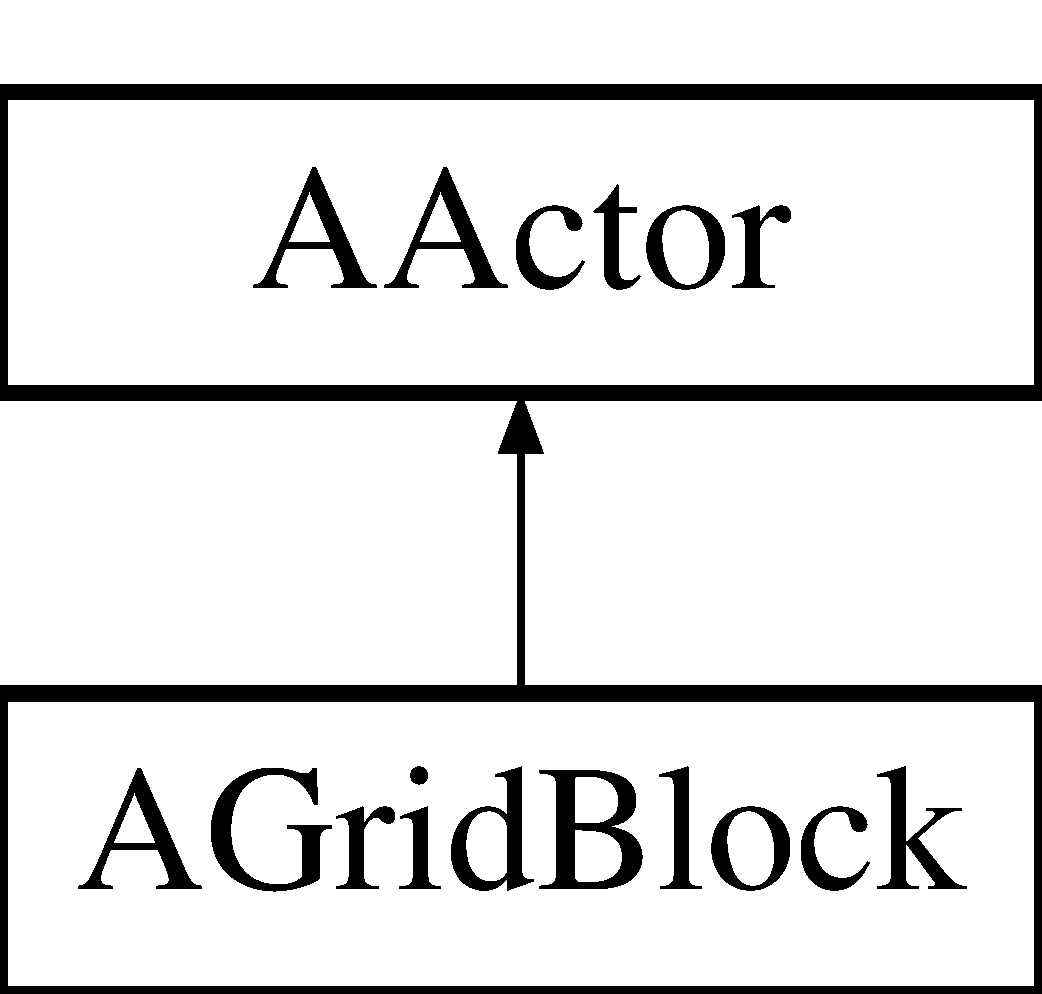
\includegraphics[height=2.000000cm]{class_a_grid_block}
\end{center}
\end{figure}
\subsection*{Public Member Functions}
\begin{DoxyCompactItemize}
\item 
void \hyperlink{class_a_grid_block_a359898585d272e8d3ca0216f880d3d25}{Block\+Clicked} (U\+Primitive\+Component $\ast$Clicked\+Comp, F\+Key Button\+Clicked)
\begin{DoxyCompactList}\small\item\em A public member taking in two variables. \end{DoxyCompactList}\item 
void \hyperlink{class_a_grid_block_adb85baf2109b5a97d951b999b2890524}{On\+Finger\+Pressed\+Block} (E\+Touch\+Index\+::\+Type Finger\+Index, U\+Primitive\+Component $\ast$Touched\+Component)
\begin{DoxyCompactList}\small\item\em A public member taking in two variables. \end{DoxyCompactList}\item 
void \hyperlink{class_a_grid_block_aab961b92795d28c156b9a64bf4936e36}{Handle\+Clicked} ()
\begin{DoxyCompactList}\small\item\em A public member. \end{DoxyCompactList}\item 
\hypertarget{class_a_grid_block_a7f649750d4be151d29f98a7c5bc898ad}{}\label{class_a_grid_block_a7f649750d4be151d29f98a7c5bc898ad} 
void {\bfseries Highlight} (bool b\+On)
\item 
F\+O\+R\+C\+E\+I\+N\+L\+I\+NE class U\+Scene\+Component $\ast$ \hyperlink{class_a_grid_block_a666f4929d04306cbe30f437d8f9f94a4}{Get\+Dummy\+Root} () const
\begin{DoxyCompactList}\small\item\em A public member taking. \end{DoxyCompactList}\item 
F\+O\+R\+C\+E\+I\+N\+L\+I\+NE class U\+Static\+Mesh\+Component $\ast$ \hyperlink{class_a_grid_block_a88866015576480a21a82b9de762cfacf}{Get\+Block\+Mesh} () const
\begin{DoxyCompactList}\small\item\em A public member. \end{DoxyCompactList}\end{DoxyCompactItemize}
\subsection*{Public Attributes}
\begin{DoxyCompactItemize}
\item 
bool \hyperlink{class_a_grid_block_a60c1ca6cb04e583147be45b85e3a1831}{b\+Is\+Active}
\begin{DoxyCompactList}\small\item\em A public variable. \end{DoxyCompactList}\item 
class U\+Material $\ast$ \hyperlink{class_a_grid_block_a30a0b537773f34ab41c2881f8e124f3a}{Base\+Material}
\begin{DoxyCompactList}\small\item\em A public variable. \end{DoxyCompactList}\item 
class U\+Material\+Instance $\ast$ \hyperlink{class_a_grid_block_a5687a984bdcb701c04af87d875c27e1f}{Blue\+Material}
\begin{DoxyCompactList}\small\item\em A public variable. \end{DoxyCompactList}\item 
class U\+Material\+Instance $\ast$ \hyperlink{class_a_grid_block_a4a396f418bffcef7a96b40e387cfd927}{Orange\+Material}
\begin{DoxyCompactList}\small\item\em A public variable. \end{DoxyCompactList}\item 
class \hyperlink{class_a_unreal_grid}{A\+Unreal\+Grid} $\ast$ \hyperlink{class_a_grid_block_af3dc096c5f96aba9b3b882f3f11deb93}{Owning\+Grid}
\begin{DoxyCompactList}\small\item\em A public variable. \end{DoxyCompactList}\item 
uint32 \hyperlink{class_a_grid_block_a8050ae31d3015e14fcae9d553977cea1}{x}
\begin{DoxyCompactList}\small\item\em A public variable. \end{DoxyCompactList}\item 
uint32 \hyperlink{class_a_grid_block_aad833bb2a47f65ef3cbba7940687c819}{y}
\begin{DoxyCompactList}\small\item\em A public variable. \end{DoxyCompactList}\end{DoxyCompactItemize}


\subsection{Detailed Description}
Class for clickable blocks. 

A class that defines clickable blocks 

\subsection{Member Function Documentation}
\hypertarget{class_a_grid_block_a359898585d272e8d3ca0216f880d3d25}{}\label{class_a_grid_block_a359898585d272e8d3ca0216f880d3d25} 
\index{A\+Grid\+Block@{A\+Grid\+Block}!Block\+Clicked@{Block\+Clicked}}
\index{Block\+Clicked@{Block\+Clicked}!A\+Grid\+Block@{A\+Grid\+Block}}
\subsubsection{\texorpdfstring{Block\+Clicked()}{BlockClicked()}}
{\footnotesize\ttfamily void A\+Grid\+Block\+::\+Block\+Clicked (\begin{DoxyParamCaption}\item[{U\+Primitive\+Component $\ast$}]{Clicked\+Comp,  }\item[{F\+Key}]{Button\+Clicked }\end{DoxyParamCaption})}



A public member taking in two variables. 

/param Clicked\+Comp the component that does the clicking /param Button\+Clicked Clicked button Handle the block being clicked. \hypertarget{class_a_grid_block_a88866015576480a21a82b9de762cfacf}{}\label{class_a_grid_block_a88866015576480a21a82b9de762cfacf} 
\index{A\+Grid\+Block@{A\+Grid\+Block}!Get\+Block\+Mesh@{Get\+Block\+Mesh}}
\index{Get\+Block\+Mesh@{Get\+Block\+Mesh}!A\+Grid\+Block@{A\+Grid\+Block}}
\subsubsection{\texorpdfstring{Get\+Block\+Mesh()}{GetBlockMesh()}}
{\footnotesize\ttfamily F\+O\+R\+C\+E\+I\+N\+L\+I\+NE class U\+Static\+Mesh\+Component$\ast$ A\+Grid\+Block\+::\+Get\+Block\+Mesh (\begin{DoxyParamCaption}{ }\end{DoxyParamCaption}) const\hspace{0.3cm}{\ttfamily [inline]}}



A public member. 

Returns Block\+Mesh subobject. \hypertarget{class_a_grid_block_a666f4929d04306cbe30f437d8f9f94a4}{}\label{class_a_grid_block_a666f4929d04306cbe30f437d8f9f94a4} 
\index{A\+Grid\+Block@{A\+Grid\+Block}!Get\+Dummy\+Root@{Get\+Dummy\+Root}}
\index{Get\+Dummy\+Root@{Get\+Dummy\+Root}!A\+Grid\+Block@{A\+Grid\+Block}}
\subsubsection{\texorpdfstring{Get\+Dummy\+Root()}{GetDummyRoot()}}
{\footnotesize\ttfamily F\+O\+R\+C\+E\+I\+N\+L\+I\+NE class U\+Scene\+Component$\ast$ A\+Grid\+Block\+::\+Get\+Dummy\+Root (\begin{DoxyParamCaption}{ }\end{DoxyParamCaption}) const\hspace{0.3cm}{\ttfamily [inline]}}



A public member taking. 

Returns Dummy\+Root subobject. \hypertarget{class_a_grid_block_aab961b92795d28c156b9a64bf4936e36}{}\label{class_a_grid_block_aab961b92795d28c156b9a64bf4936e36} 
\index{A\+Grid\+Block@{A\+Grid\+Block}!Handle\+Clicked@{Handle\+Clicked}}
\index{Handle\+Clicked@{Handle\+Clicked}!A\+Grid\+Block@{A\+Grid\+Block}}
\subsubsection{\texorpdfstring{Handle\+Clicked()}{HandleClicked()}}
{\footnotesize\ttfamily void A\+Grid\+Block\+::\+Handle\+Clicked (\begin{DoxyParamCaption}{ }\end{DoxyParamCaption})}



A public member. 

Handle Clicks on grid. \hypertarget{class_a_grid_block_adb85baf2109b5a97d951b999b2890524}{}\label{class_a_grid_block_adb85baf2109b5a97d951b999b2890524} 
\index{A\+Grid\+Block@{A\+Grid\+Block}!On\+Finger\+Pressed\+Block@{On\+Finger\+Pressed\+Block}}
\index{On\+Finger\+Pressed\+Block@{On\+Finger\+Pressed\+Block}!A\+Grid\+Block@{A\+Grid\+Block}}
\subsubsection{\texorpdfstring{On\+Finger\+Pressed\+Block()}{OnFingerPressedBlock()}}
{\footnotesize\ttfamily void A\+Grid\+Block\+::\+On\+Finger\+Pressed\+Block (\begin{DoxyParamCaption}\item[{E\+Touch\+Index\+::\+Type}]{Finger\+Index,  }\item[{U\+Primitive\+Component $\ast$}]{Touched\+Component }\end{DoxyParamCaption})}



A public member taking in two variables. 

/param Finger\+Index touch index /param Touched\+Component the component that handles touch Handle the block being touched. 

\subsection{Member Data Documentation}
\hypertarget{class_a_grid_block_a30a0b537773f34ab41c2881f8e124f3a}{}\label{class_a_grid_block_a30a0b537773f34ab41c2881f8e124f3a} 
\index{A\+Grid\+Block@{A\+Grid\+Block}!Base\+Material@{Base\+Material}}
\index{Base\+Material@{Base\+Material}!A\+Grid\+Block@{A\+Grid\+Block}}
\subsubsection{\texorpdfstring{Base\+Material}{BaseMaterial}}
{\footnotesize\ttfamily class U\+Material$\ast$ A\+Grid\+Block\+::\+Base\+Material}



A public variable. 

Pointer to white material used on the focused block \hypertarget{class_a_grid_block_a60c1ca6cb04e583147be45b85e3a1831}{}\label{class_a_grid_block_a60c1ca6cb04e583147be45b85e3a1831} 
\index{A\+Grid\+Block@{A\+Grid\+Block}!b\+Is\+Active@{b\+Is\+Active}}
\index{b\+Is\+Active@{b\+Is\+Active}!A\+Grid\+Block@{A\+Grid\+Block}}
\subsubsection{\texorpdfstring{b\+Is\+Active}{bIsActive}}
{\footnotesize\ttfamily bool A\+Grid\+Block\+::b\+Is\+Active}



A public variable. 

Are we currently active? \hypertarget{class_a_grid_block_a5687a984bdcb701c04af87d875c27e1f}{}\label{class_a_grid_block_a5687a984bdcb701c04af87d875c27e1f} 
\index{A\+Grid\+Block@{A\+Grid\+Block}!Blue\+Material@{Blue\+Material}}
\index{Blue\+Material@{Blue\+Material}!A\+Grid\+Block@{A\+Grid\+Block}}
\subsubsection{\texorpdfstring{Blue\+Material}{BlueMaterial}}
{\footnotesize\ttfamily class U\+Material\+Instance$\ast$ A\+Grid\+Block\+::\+Blue\+Material}



A public variable. 

Pointer to blue material used on inactive blocks \hypertarget{class_a_grid_block_a4a396f418bffcef7a96b40e387cfd927}{}\label{class_a_grid_block_a4a396f418bffcef7a96b40e387cfd927} 
\index{A\+Grid\+Block@{A\+Grid\+Block}!Orange\+Material@{Orange\+Material}}
\index{Orange\+Material@{Orange\+Material}!A\+Grid\+Block@{A\+Grid\+Block}}
\subsubsection{\texorpdfstring{Orange\+Material}{OrangeMaterial}}
{\footnotesize\ttfamily class U\+Material\+Instance$\ast$ A\+Grid\+Block\+::\+Orange\+Material}



A public variable. 

Pointer to orange material used on active blocks \hypertarget{class_a_grid_block_af3dc096c5f96aba9b3b882f3f11deb93}{}\label{class_a_grid_block_af3dc096c5f96aba9b3b882f3f11deb93} 
\index{A\+Grid\+Block@{A\+Grid\+Block}!Owning\+Grid@{Owning\+Grid}}
\index{Owning\+Grid@{Owning\+Grid}!A\+Grid\+Block@{A\+Grid\+Block}}
\subsubsection{\texorpdfstring{Owning\+Grid}{OwningGrid}}
{\footnotesize\ttfamily class \hyperlink{class_a_unreal_grid}{A\+Unreal\+Grid}$\ast$ A\+Grid\+Block\+::\+Owning\+Grid}



A public variable. 

\hyperlink{class_grid}{Grid} that owns us \hypertarget{class_a_grid_block_a8050ae31d3015e14fcae9d553977cea1}{}\label{class_a_grid_block_a8050ae31d3015e14fcae9d553977cea1} 
\index{A\+Grid\+Block@{A\+Grid\+Block}!x@{x}}
\index{x@{x}!A\+Grid\+Block@{A\+Grid\+Block}}
\subsubsection{\texorpdfstring{x}{x}}
{\footnotesize\ttfamily uint32 A\+Grid\+Block\+::x}



A public variable. 

X-\/co-\/ordinate \hypertarget{class_a_grid_block_aad833bb2a47f65ef3cbba7940687c819}{}\label{class_a_grid_block_aad833bb2a47f65ef3cbba7940687c819} 
\index{A\+Grid\+Block@{A\+Grid\+Block}!y@{y}}
\index{y@{y}!A\+Grid\+Block@{A\+Grid\+Block}}
\subsubsection{\texorpdfstring{y}{y}}
{\footnotesize\ttfamily uint32 A\+Grid\+Block\+::y}



A public variable. 

Y-\/co-\/ordinate 

The documentation for this class was generated from the following files\+:\begin{DoxyCompactItemize}
\item 
Grid\+Block.\+h\item 
Grid\+Block.\+cpp\end{DoxyCompactItemize}

\hypertarget{class_a_unit2_d}{}\section{A\+Unit2D Class Reference}
\label{class_a_unit2_d}\index{A\+Unit2D@{A\+Unit2D}}


Class for Units in the game.  




{\ttfamily \#include $<$Unit2\+D.\+h$>$}

Inheritance diagram for A\+Unit2D\+:\begin{figure}[H]
\begin{center}
\leavevmode
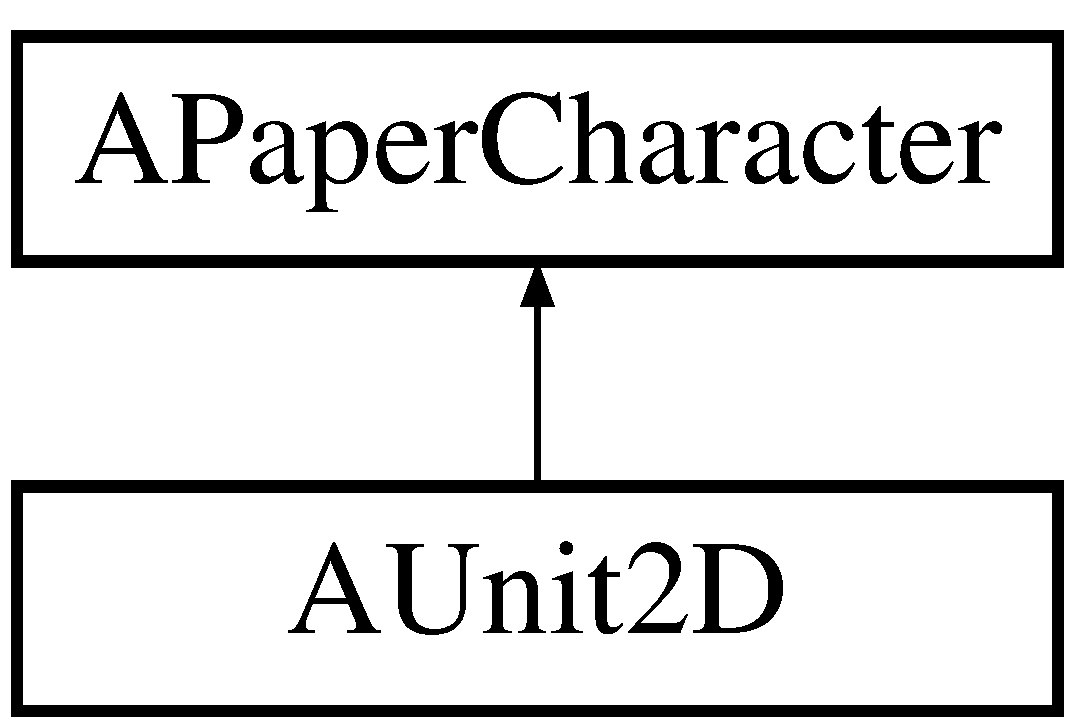
\includegraphics[height=2.000000cm]{class_a_unit2_d}
\end{center}
\end{figure}
\subsection*{Public Member Functions}
\begin{DoxyCompactItemize}
\item 
virtual void \hyperlink{class_a_unit2_d_a0251a37e303fe179ac987203df3b4f2f}{Begin\+Play} () override
\begin{DoxyCompactList}\small\item\em Inherited Member. \end{DoxyCompactList}\item 
virtual void \hyperlink{class_a_unit2_d_aabcd72dc2ba9d71a56e58148382607b2}{Tick} (float Delta\+Seconds) override
\begin{DoxyCompactList}\small\item\em Inherited Member. \end{DoxyCompactList}\item 
virtual void \hyperlink{class_a_unit2_d_ae5ce5587eb783da80ed36f7b55724a56}{Setup\+Player\+Input\+Component} (class U\+Input\+Component $\ast$Input\+Component) override
\begin{DoxyCompactList}\small\item\em Inherited Member. \end{DoxyCompactList}\item 
void \hyperlink{class_a_unit2_d_a6a1a7ef96c7efebf5a7f50b011b7a6c0}{Handle\+Left\+Click} ()
\begin{DoxyCompactList}\small\item\em A normal member. \end{DoxyCompactList}\item 
void \hyperlink{class_a_unit2_d_a96e805c919d9088872a5c8945a9ca31f}{cancel} ()
\begin{DoxyCompactList}\small\item\em A normal member. \end{DoxyCompactList}\item 
\hyperlink{class_a_unit2_d}{A\+Unit2D} $\ast$ \hyperlink{class_a_unit2_d_ab9a04722aeaa02b1d656c2ea7c6bdad2}{Find\+Focused\+Target} ()
\begin{DoxyCompactList}\small\item\em A normal member returning a Unit2D object. \end{DoxyCompactList}\item 
bool \hyperlink{class_a_unit2_d_a6426fb6d603a376b3808d558cf07c17e}{get\+Side} ()
\begin{DoxyCompactList}\small\item\em A normal member. \end{DoxyCompactList}\item 
int32 \hyperlink{class_a_unit2_d_a5f1d562d11394d02ad291e7cdfaa159b}{get\+HP} ()
\begin{DoxyCompactList}\small\item\em A normal member returning an integer value. \end{DoxyCompactList}\item 
int32 \hyperlink{class_a_unit2_d_a0e21fbf4b83553f9910b4dd9a28ba2fb}{get\+A\+CC} ()
\begin{DoxyCompactList}\small\item\em A normal member returning an integer value. \end{DoxyCompactList}\item 
int32 \hyperlink{class_a_unit2_d_aa66921015cf3b796869bd23fddcc162b}{get\+R\+FL} ()
\begin{DoxyCompactList}\small\item\em A normal member returning an integer value. \end{DoxyCompactList}\item 
int32 \hyperlink{class_a_unit2_d_adbe5785b68849e82ab11c48f86df64e7}{get\+TU} ()
\begin{DoxyCompactList}\small\item\em A normal member returning an integer value. \end{DoxyCompactList}\item 
int32 \hyperlink{class_a_unit2_d_a484b69b741bb37babd27306fbfc5990b}{get\+B\+RV} ()
\begin{DoxyCompactList}\small\item\em A normal member returning an integer value. \end{DoxyCompactList}\item 
void \hyperlink{class_a_unit2_d_a60a8c2a02713d1fb838757a2b74c0d5b}{set\+HP} (int32 hp)
\begin{DoxyCompactList}\small\item\em A normal member. \end{DoxyCompactList}\item 
void \hyperlink{class_a_unit2_d_a6c9367b81fabd482ded876c47e006d35}{set\+A\+CC} (int32 acc)
\begin{DoxyCompactList}\small\item\em A normal member. \end{DoxyCompactList}\item 
void \hyperlink{class_a_unit2_d_a1f444ba247643672bec2a87beec14fb0}{set\+R\+FL} (int32 rfl)
\begin{DoxyCompactList}\small\item\em A normal member. \end{DoxyCompactList}\item 
void \hyperlink{class_a_unit2_d_ac7e18514213510c0077518ab1052340a}{set\+TU} (int32 tu)
\begin{DoxyCompactList}\small\item\em A normal member. \end{DoxyCompactList}\item 
void \hyperlink{class_a_unit2_d_a6a1ed9c8a68c9954bb88c58539250f87}{set\+B\+RV} (int32 brv)
\begin{DoxyCompactList}\small\item\em A normal member. \end{DoxyCompactList}\item 
void \hyperlink{class_a_unit2_d_a8567eec6dc49533041735e125cace6e2}{move} ()
\begin{DoxyCompactList}\small\item\em A normal member. \end{DoxyCompactList}\item 
\hypertarget{class_a_unit2_d_a00227806480536a3b6f34eed9529e173}{}\label{class_a_unit2_d_a00227806480536a3b6f34eed9529e173} 
void {\bfseries hit} ()
\item 
void \hyperlink{class_a_unit2_d_a3a66da88663696462e73a5933c0d1032}{change\+State} (E\+Unit\+State \hyperlink{class_a_unit2_d_a33b3a09dc710021ce343630e828ebb1b}{state})
\begin{DoxyCompactList}\small\item\em A normal member. \end{DoxyCompactList}\item 
void \hyperlink{class_a_unit2_d_a6631cea7c02eb12361dc14439b942f70}{frag\+Grenade} ()
\begin{DoxyCompactList}\small\item\em A normal member. \end{DoxyCompactList}\item 
void \hyperlink{class_a_unit2_d_ae12beff66c2558df2ca19ae222900988}{smoke\+Grenade} ()
\begin{DoxyCompactList}\small\item\em A normal member. \end{DoxyCompactList}\item 
void \hyperlink{class_a_unit2_d_af14e1b38ce6238bb9343eca175c15f29}{flashbang\+Grenade} ()
\begin{DoxyCompactList}\small\item\em A normal member. \end{DoxyCompactList}\item 
void \hyperlink{class_a_unit2_d_a9ba62a68377a9584eee863d76079943b}{flash} ()
\begin{DoxyCompactList}\small\item\em A normal member. \end{DoxyCompactList}\item 
void \hyperlink{class_a_unit2_d_a895149436f783d3c0bbfe80556196438}{reset\+Frag} ()
\begin{DoxyCompactList}\small\item\em A normal member. \end{DoxyCompactList}\item 
void \hyperlink{class_a_unit2_d_a80ad176a4ed566c1fb18df231290c8b4}{reset\+Smoke} ()
\begin{DoxyCompactList}\small\item\em A normal member. \end{DoxyCompactList}\item 
void \hyperlink{class_a_unit2_d_a509be02c409aec4f9db70eedc954dec8}{reset\+Flashbang} ()
\begin{DoxyCompactList}\small\item\em A normal member. \end{DoxyCompactList}\item 
void \hyperlink{class_a_unit2_d_a6cbf098b221157bb99dc278b3c8dab70}{shoot} ()
\begin{DoxyCompactList}\small\item\em A normal member. \end{DoxyCompactList}\item 
void \hyperlink{class_a_unit2_d_a4e21cbdac89dcc72f670ad77dfc474cb}{reload} ()
\begin{DoxyCompactList}\small\item\em A normal member. \end{DoxyCompactList}\item 
bool \hyperlink{class_a_unit2_d_aec8aadc1698c1a0e26d76ce97b2515d0}{determine\+Hit} (\hyperlink{class_a_unit2_d}{A\+Unit2D} $\ast$target)
\begin{DoxyCompactList}\small\item\em A normal member taking an argument and returning a boolean value. \end{DoxyCompactList}\item 
void \hyperlink{class_a_unit2_d_a383ec068bf651417a27c4e7f9a44ce1c}{take\+Damage} (int damage)
\begin{DoxyCompactList}\small\item\em A normal member taking an argument. \end{DoxyCompactList}\item 
void \hyperlink{class_a_unit2_d_aa98e4af27fd175f81fc9761e4b139caf}{stun} ()
\begin{DoxyCompactList}\small\item\em A normal member. \end{DoxyCompactList}\item 
void \hyperlink{class_a_unit2_d_a141b33f9f1c9409e645960903ccb714f}{reset\+TU} ()
\begin{DoxyCompactList}\small\item\em A normal member. \end{DoxyCompactList}\item 
void \hyperlink{class_a_unit2_d_af13c789a87a18daa455387f44d84d333}{set\+Percent\+Health} ()
\begin{DoxyCompactList}\small\item\em A normal member. \end{DoxyCompactList}\item 
void \hyperlink{class_a_unit2_d_a0f93d2f4547813149e5b46530dcaba67}{set\+Percent\+TU} ()
\begin{DoxyCompactList}\small\item\em A normal member. \end{DoxyCompactList}\item 
void \hyperlink{class_a_unit2_d_a30c4c53f8789064bb9fc7b7d8703ae35}{set\+Percent\+B\+RV} ()
\begin{DoxyCompactList}\small\item\em A normal member. \end{DoxyCompactList}\item 
void \hyperlink{class_a_unit2_d_ae1d7c09760d899ca25e96a9573b2ddf0}{check\+Freakout} ()
\begin{DoxyCompactList}\small\item\em A normal member. \end{DoxyCompactList}\item 
void \hyperlink{class_a_unit2_d_aa0a382d42b3024c460e549054b158803}{run} ()
\begin{DoxyCompactList}\small\item\em A normal member. \end{DoxyCompactList}\item 
void \hyperlink{class_a_unit2_d_ae1e36f7fa10bf392c4ceb150fd6addc8}{hunker\+Down} ()
\begin{DoxyCompactList}\small\item\em A normal member. \end{DoxyCompactList}\end{DoxyCompactItemize}
\subsection*{Public Attributes}
\begin{DoxyCompactItemize}
\item 
E\+Unit\+State \hyperlink{class_a_unit2_d_a33b3a09dc710021ce343630e828ebb1b}{state} = E\+Unit\+State\+::\+U\+S\+\_\+\+Idle
\begin{DoxyCompactList}\small\item\em A public variable. \end{DoxyCompactList}\end{DoxyCompactItemize}
\subsection*{Protected Attributes}
\begin{DoxyCompactItemize}
\item 
class U\+Paper\+Sprite\+Component $\ast$ \hyperlink{class_a_unit2_d_a03b2c6b3e63c261e81b5a193ed0d4acd}{sprite\+Comp}
\begin{DoxyCompactList}\small\item\em A protected variable. \end{DoxyCompactList}\item 
class U\+Paper\+Flipbook $\ast$ \hyperlink{class_a_unit2_d_a1c7ee8387eeb37c2c1f735b61135865d}{Idle\+Animation}
\begin{DoxyCompactList}\small\item\em A protected variable. \end{DoxyCompactList}\item 
bool \hyperlink{class_a_unit2_d_ab916af70c15214293b1f868ef61538e2}{is\+Player\+One} = true
\begin{DoxyCompactList}\small\item\em A protected variable. \end{DoxyCompactList}\item 
int32 \hyperlink{class_a_unit2_d_a251c25f80c0fe087b892d82baf8cfa0d}{health\+Point} = 20
\begin{DoxyCompactList}\small\item\em A protected variable. \end{DoxyCompactList}\item 
int32 \hyperlink{class_a_unit2_d_a7c93157ba7198cdb15bde2e3b649988d}{max\+Health} = 40
\begin{DoxyCompactList}\small\item\em A protected variable. \end{DoxyCompactList}\item 
float \hyperlink{class_a_unit2_d_a731e52449dba6368b509b78ac95c0dc0}{percent\+Health} = \hyperlink{class_a_unit2_d_a251c25f80c0fe087b892d82baf8cfa0d}{health\+Point}$\ast$1.\+0/\hyperlink{class_a_unit2_d_a7c93157ba7198cdb15bde2e3b649988d}{max\+Health}
\begin{DoxyCompactList}\small\item\em A protected variable. \end{DoxyCompactList}\item 
int32 \hyperlink{class_a_unit2_d_a24f6252522a9d97f9ea8ea9cbf6cca69}{current\+Time\+Unit} = 50
\begin{DoxyCompactList}\small\item\em A protected variable. \end{DoxyCompactList}\item 
int32 \hyperlink{class_a_unit2_d_a0a8041a5fc46bd09fed79303fbcd3ce5}{max\+Time\+Unit} = 50
\begin{DoxyCompactList}\small\item\em A protected variable. \end{DoxyCompactList}\item 
float \hyperlink{class_a_unit2_d_a45d8a7f3f28c1a641dd4124c4b7ba272}{percent\+TU} = \hyperlink{class_a_unit2_d_a24f6252522a9d97f9ea8ea9cbf6cca69}{current\+Time\+Unit}$\ast$1.\+0 / \hyperlink{class_a_unit2_d_a0a8041a5fc46bd09fed79303fbcd3ce5}{max\+Time\+Unit}
\begin{DoxyCompactList}\small\item\em A protected variable. \end{DoxyCompactList}\item 
int32 \hyperlink{class_a_unit2_d_a639a503e506215b11c81167154bf9bfd}{accuracy} = 40
\begin{DoxyCompactList}\small\item\em A protected variable. \end{DoxyCompactList}\item 
int32 \hyperlink{class_a_unit2_d_a178510f321f19d1fa8b19b1a16b7dcfb}{reflex} = 55
\begin{DoxyCompactList}\small\item\em A protected variable. \end{DoxyCompactList}\item 
int32 \hyperlink{class_a_unit2_d_a5e26bf8a80a9363d3538b1e1f675fb61}{max\+Bravery} = 65
\begin{DoxyCompactList}\small\item\em A protected variable. \end{DoxyCompactList}\item 
int32 \hyperlink{class_a_unit2_d_aee9f4f0703e027df353d51811befb1c3}{current\+Bravery} = 65
\begin{DoxyCompactList}\small\item\em A protected variable. \end{DoxyCompactList}\item 
float \hyperlink{class_a_unit2_d_a837bd3a0faaf2ebd2796de9a16da8fa0}{percent\+Brv} = \hyperlink{class_a_unit2_d_aee9f4f0703e027df353d51811befb1c3}{current\+Bravery}$\ast$1.\+0/ \hyperlink{class_a_unit2_d_a5e26bf8a80a9363d3538b1e1f675fb61}{max\+Bravery}
\begin{DoxyCompactList}\small\item\em A protected variable. \end{DoxyCompactList}\item 
int32 \hyperlink{class_a_unit2_d_a7947b8f9bed2225ed223f37f21820960}{clip\+Size} = 12
\begin{DoxyCompactList}\small\item\em A protected variable. \end{DoxyCompactList}\item 
int32 \hyperlink{class_a_unit2_d_a7f23a4544c24d5fd0489f2420a7b3eb4}{bullet} = \hyperlink{class_a_unit2_d_a7947b8f9bed2225ed223f37f21820960}{clip\+Size}
\begin{DoxyCompactList}\small\item\em A protected variable. \end{DoxyCompactList}\item 
int32 \hyperlink{class_a_unit2_d_ad2d855d2c78d2e1918b84df6ae4da192}{frag} = 2
\begin{DoxyCompactList}\small\item\em A protected variable. \end{DoxyCompactList}\item 
int32 \hyperlink{class_a_unit2_d_a898e4c6cf4c37c9a1b84d73a7fb30c6b}{flashbang} = 2
\begin{DoxyCompactList}\small\item\em A protected variable. \end{DoxyCompactList}\item 
int32 \hyperlink{class_a_unit2_d_a6cfd32ab7bfaa5dbc64defd1f74bf459}{smoke} = 2
\begin{DoxyCompactList}\small\item\em A protected variable. \end{DoxyCompactList}\item 
int32 \hyperlink{class_a_unit2_d_a583df0bd3be284fddf24c1c627053767}{weapon\+Dmg} = 20
\begin{DoxyCompactList}\small\item\em A protected variable. \end{DoxyCompactList}\item 
float \hyperlink{class_a_unit2_d_a6945ed1b7f56335e3c42d414f9e9b243}{range\+Falloff}
\begin{DoxyCompactList}\small\item\em A protected variable. \end{DoxyCompactList}\item 
int32 \hyperlink{class_a_unit2_d_ab8a5bca2e21f1c992b887646d19a7025}{weapon\+Cost} = 32
\begin{DoxyCompactList}\small\item\em A protected variable. \end{DoxyCompactList}\end{DoxyCompactItemize}


\subsection{Detailed Description}
Class for Units in the game. 

An Unreal Paper2D class that defines Units in the game. The class contains Unit Statistics such as HP, TU, R\+FL, A\+CC, and B\+RV, as well as weapon statistics such as damage and ammo count. The Unit2D class also inherits unreal functions for characters and contains functions to handle interactions with other Unit2D objects. Unit2D also handles controls for its own object. 

\subsection{Member Function Documentation}
\hypertarget{class_a_unit2_d_a0251a37e303fe179ac987203df3b4f2f}{}\label{class_a_unit2_d_a0251a37e303fe179ac987203df3b4f2f} 
\index{A\+Unit2D@{A\+Unit2D}!Begin\+Play@{Begin\+Play}}
\index{Begin\+Play@{Begin\+Play}!A\+Unit2D@{A\+Unit2D}}
\subsubsection{\texorpdfstring{Begin\+Play()}{BeginPlay()}}
{\footnotesize\ttfamily void A\+Unit2\+D\+::\+Begin\+Play (\begin{DoxyParamCaption}{ }\end{DoxyParamCaption})\hspace{0.3cm}{\ttfamily [override]}, {\ttfamily [virtual]}}



Inherited Member. 

Inherited Begin, called when the game starts or when spawned \hypertarget{class_a_unit2_d_a96e805c919d9088872a5c8945a9ca31f}{}\label{class_a_unit2_d_a96e805c919d9088872a5c8945a9ca31f} 
\index{A\+Unit2D@{A\+Unit2D}!cancel@{cancel}}
\index{cancel@{cancel}!A\+Unit2D@{A\+Unit2D}}
\subsubsection{\texorpdfstring{cancel()}{cancel()}}
{\footnotesize\ttfamily void A\+Unit2\+D\+::cancel (\begin{DoxyParamCaption}{ }\end{DoxyParamCaption})}



A normal member. 

method for resetting the palyer state back to idle \hypertarget{class_a_unit2_d_a3a66da88663696462e73a5933c0d1032}{}\label{class_a_unit2_d_a3a66da88663696462e73a5933c0d1032} 
\index{A\+Unit2D@{A\+Unit2D}!change\+State@{change\+State}}
\index{change\+State@{change\+State}!A\+Unit2D@{A\+Unit2D}}
\subsubsection{\texorpdfstring{change\+State()}{changeState()}}
{\footnotesize\ttfamily void A\+Unit2\+D\+::change\+State (\begin{DoxyParamCaption}\item[{E\+Unit\+State}]{state }\end{DoxyParamCaption})}



A normal member. 


\begin{DoxyParams}{Parameters}
{\em state} & new unit state to set to A method to change the current state of the unit. \\
\hline
\end{DoxyParams}
\hypertarget{class_a_unit2_d_ae1d7c09760d899ca25e96a9573b2ddf0}{}\label{class_a_unit2_d_ae1d7c09760d899ca25e96a9573b2ddf0} 
\index{A\+Unit2D@{A\+Unit2D}!check\+Freakout@{check\+Freakout}}
\index{check\+Freakout@{check\+Freakout}!A\+Unit2D@{A\+Unit2D}}
\subsubsection{\texorpdfstring{check\+Freakout()}{checkFreakout()}}
{\footnotesize\ttfamily void A\+Unit2\+D\+::check\+Freakout (\begin{DoxyParamCaption}{ }\end{DoxyParamCaption})}



A normal member. 

Check if the unit freaksout based on bravery score. \hypertarget{class_a_unit2_d_aec8aadc1698c1a0e26d76ce97b2515d0}{}\label{class_a_unit2_d_aec8aadc1698c1a0e26d76ce97b2515d0} 
\index{A\+Unit2D@{A\+Unit2D}!determine\+Hit@{determine\+Hit}}
\index{determine\+Hit@{determine\+Hit}!A\+Unit2D@{A\+Unit2D}}
\subsubsection{\texorpdfstring{determine\+Hit()}{determineHit()}}
{\footnotesize\ttfamily bool A\+Unit2\+D\+::determine\+Hit (\begin{DoxyParamCaption}\item[{\hyperlink{class_a_unit2_d}{A\+Unit2D} $\ast$}]{target }\end{DoxyParamCaption})}



A normal member taking an argument and returning a boolean value. 


\begin{DoxyParams}{Parameters}
{\em target} & pointer to another Unit2D object Determine if an attack will hit the target. \\
\hline
\end{DoxyParams}
\hypertarget{class_a_unit2_d_ab9a04722aeaa02b1d656c2ea7c6bdad2}{}\label{class_a_unit2_d_ab9a04722aeaa02b1d656c2ea7c6bdad2} 
\index{A\+Unit2D@{A\+Unit2D}!Find\+Focused\+Target@{Find\+Focused\+Target}}
\index{Find\+Focused\+Target@{Find\+Focused\+Target}!A\+Unit2D@{A\+Unit2D}}
\subsubsection{\texorpdfstring{Find\+Focused\+Target()}{FindFocusedTarget()}}
{\footnotesize\ttfamily \hyperlink{class_a_unit2_d}{A\+Unit2D} $\ast$ A\+Unit2\+D\+::\+Find\+Focused\+Target (\begin{DoxyParamCaption}{ }\end{DoxyParamCaption})}



A normal member returning a Unit2D object. 

method for returning a Unit2D object that has been moused over \hypertarget{class_a_unit2_d_a9ba62a68377a9584eee863d76079943b}{}\label{class_a_unit2_d_a9ba62a68377a9584eee863d76079943b} 
\index{A\+Unit2D@{A\+Unit2D}!flash@{flash}}
\index{flash@{flash}!A\+Unit2D@{A\+Unit2D}}
\subsubsection{\texorpdfstring{flash()}{flash()}}
{\footnotesize\ttfamily void A\+Unit2\+D\+::flash (\begin{DoxyParamCaption}{ }\end{DoxyParamCaption})}



A normal member. 

A method for handling the effects of a flashbang. \hypertarget{class_a_unit2_d_af14e1b38ce6238bb9343eca175c15f29}{}\label{class_a_unit2_d_af14e1b38ce6238bb9343eca175c15f29} 
\index{A\+Unit2D@{A\+Unit2D}!flashbang\+Grenade@{flashbang\+Grenade}}
\index{flashbang\+Grenade@{flashbang\+Grenade}!A\+Unit2D@{A\+Unit2D}}
\subsubsection{\texorpdfstring{flashbang\+Grenade()}{flashbangGrenade()}}
{\footnotesize\ttfamily void A\+Unit2\+D\+::flashbang\+Grenade (\begin{DoxyParamCaption}{ }\end{DoxyParamCaption})}



A normal member. 

A method for handling the action of throwing a Flashbang grenade. \hypertarget{class_a_unit2_d_a6631cea7c02eb12361dc14439b942f70}{}\label{class_a_unit2_d_a6631cea7c02eb12361dc14439b942f70} 
\index{A\+Unit2D@{A\+Unit2D}!frag\+Grenade@{frag\+Grenade}}
\index{frag\+Grenade@{frag\+Grenade}!A\+Unit2D@{A\+Unit2D}}
\subsubsection{\texorpdfstring{frag\+Grenade()}{fragGrenade()}}
{\footnotesize\ttfamily void A\+Unit2\+D\+::frag\+Grenade (\begin{DoxyParamCaption}{ }\end{DoxyParamCaption})}



A normal member. 

A method for handling the action of throwing a frag grenade. \hypertarget{class_a_unit2_d_a0e21fbf4b83553f9910b4dd9a28ba2fb}{}\label{class_a_unit2_d_a0e21fbf4b83553f9910b4dd9a28ba2fb} 
\index{A\+Unit2D@{A\+Unit2D}!get\+A\+CC@{get\+A\+CC}}
\index{get\+A\+CC@{get\+A\+CC}!A\+Unit2D@{A\+Unit2D}}
\subsubsection{\texorpdfstring{get\+A\+C\+C()}{getACC()}}
{\footnotesize\ttfamily int32 A\+Unit2\+D\+::get\+A\+CC (\begin{DoxyParamCaption}{ }\end{DoxyParamCaption})}



A normal member returning an integer value. 

getter for accuracy. \hypertarget{class_a_unit2_d_a484b69b741bb37babd27306fbfc5990b}{}\label{class_a_unit2_d_a484b69b741bb37babd27306fbfc5990b} 
\index{A\+Unit2D@{A\+Unit2D}!get\+B\+RV@{get\+B\+RV}}
\index{get\+B\+RV@{get\+B\+RV}!A\+Unit2D@{A\+Unit2D}}
\subsubsection{\texorpdfstring{get\+B\+R\+V()}{getBRV()}}
{\footnotesize\ttfamily int32 A\+Unit2\+D\+::get\+B\+RV (\begin{DoxyParamCaption}{ }\end{DoxyParamCaption})}



A normal member returning an integer value. 

getter for current bravery. \hypertarget{class_a_unit2_d_a5f1d562d11394d02ad291e7cdfaa159b}{}\label{class_a_unit2_d_a5f1d562d11394d02ad291e7cdfaa159b} 
\index{A\+Unit2D@{A\+Unit2D}!get\+HP@{get\+HP}}
\index{get\+HP@{get\+HP}!A\+Unit2D@{A\+Unit2D}}
\subsubsection{\texorpdfstring{get\+H\+P()}{getHP()}}
{\footnotesize\ttfamily int32 A\+Unit2\+D\+::get\+HP (\begin{DoxyParamCaption}{ }\end{DoxyParamCaption})}



A normal member returning an integer value. 

getter for current hp. \hypertarget{class_a_unit2_d_aa66921015cf3b796869bd23fddcc162b}{}\label{class_a_unit2_d_aa66921015cf3b796869bd23fddcc162b} 
\index{A\+Unit2D@{A\+Unit2D}!get\+R\+FL@{get\+R\+FL}}
\index{get\+R\+FL@{get\+R\+FL}!A\+Unit2D@{A\+Unit2D}}
\subsubsection{\texorpdfstring{get\+R\+F\+L()}{getRFL()}}
{\footnotesize\ttfamily int32 A\+Unit2\+D\+::get\+R\+FL (\begin{DoxyParamCaption}{ }\end{DoxyParamCaption})}



A normal member returning an integer value. 

getter for reflex. \hypertarget{class_a_unit2_d_a6426fb6d603a376b3808d558cf07c17e}{}\label{class_a_unit2_d_a6426fb6d603a376b3808d558cf07c17e} 
\index{A\+Unit2D@{A\+Unit2D}!get\+Side@{get\+Side}}
\index{get\+Side@{get\+Side}!A\+Unit2D@{A\+Unit2D}}
\subsubsection{\texorpdfstring{get\+Side()}{getSide()}}
{\footnotesize\ttfamily bool A\+Unit2\+D\+::get\+Side (\begin{DoxyParamCaption}{ }\end{DoxyParamCaption})}



A normal member. 

getter for player side. \hypertarget{class_a_unit2_d_adbe5785b68849e82ab11c48f86df64e7}{}\label{class_a_unit2_d_adbe5785b68849e82ab11c48f86df64e7} 
\index{A\+Unit2D@{A\+Unit2D}!get\+TU@{get\+TU}}
\index{get\+TU@{get\+TU}!A\+Unit2D@{A\+Unit2D}}
\subsubsection{\texorpdfstring{get\+T\+U()}{getTU()}}
{\footnotesize\ttfamily int32 A\+Unit2\+D\+::get\+TU (\begin{DoxyParamCaption}{ }\end{DoxyParamCaption})}



A normal member returning an integer value. 

getter for current time unit. \hypertarget{class_a_unit2_d_a6a1a7ef96c7efebf5a7f50b011b7a6c0}{}\label{class_a_unit2_d_a6a1a7ef96c7efebf5a7f50b011b7a6c0} 
\index{A\+Unit2D@{A\+Unit2D}!Handle\+Left\+Click@{Handle\+Left\+Click}}
\index{Handle\+Left\+Click@{Handle\+Left\+Click}!A\+Unit2D@{A\+Unit2D}}
\subsubsection{\texorpdfstring{Handle\+Left\+Click()}{HandleLeftClick()}}
{\footnotesize\ttfamily void A\+Unit2\+D\+::\+Handle\+Left\+Click (\begin{DoxyParamCaption}{ }\end{DoxyParamCaption})}



A normal member. 

used for handling left clicks, depending on the current state \hypertarget{class_a_unit2_d_ae1e36f7fa10bf392c4ceb150fd6addc8}{}\label{class_a_unit2_d_ae1e36f7fa10bf392c4ceb150fd6addc8} 
\index{A\+Unit2D@{A\+Unit2D}!hunker\+Down@{hunker\+Down}}
\index{hunker\+Down@{hunker\+Down}!A\+Unit2D@{A\+Unit2D}}
\subsubsection{\texorpdfstring{hunker\+Down()}{hunkerDown()}}
{\footnotesize\ttfamily void A\+Unit2\+D\+::hunker\+Down (\begin{DoxyParamCaption}{ }\end{DoxyParamCaption})}



A normal member. 

Handle the \char`\"{}hunker down\char`\"{} freakout. \hypertarget{class_a_unit2_d_a8567eec6dc49533041735e125cace6e2}{}\label{class_a_unit2_d_a8567eec6dc49533041735e125cace6e2} 
\index{A\+Unit2D@{A\+Unit2D}!move@{move}}
\index{move@{move}!A\+Unit2D@{A\+Unit2D}}
\subsubsection{\texorpdfstring{move()}{move()}}
{\footnotesize\ttfamily void A\+Unit2\+D\+::move (\begin{DoxyParamCaption}{ }\end{DoxyParamCaption})}



A normal member. 

move method. \hypertarget{class_a_unit2_d_a4e21cbdac89dcc72f670ad77dfc474cb}{}\label{class_a_unit2_d_a4e21cbdac89dcc72f670ad77dfc474cb} 
\index{A\+Unit2D@{A\+Unit2D}!reload@{reload}}
\index{reload@{reload}!A\+Unit2D@{A\+Unit2D}}
\subsubsection{\texorpdfstring{reload()}{reload()}}
{\footnotesize\ttfamily void A\+Unit2\+D\+::reload (\begin{DoxyParamCaption}{ }\end{DoxyParamCaption})}



A normal member. 

Reset current bullet count to the clipsize. \hypertarget{class_a_unit2_d_a509be02c409aec4f9db70eedc954dec8}{}\label{class_a_unit2_d_a509be02c409aec4f9db70eedc954dec8} 
\index{A\+Unit2D@{A\+Unit2D}!reset\+Flashbang@{reset\+Flashbang}}
\index{reset\+Flashbang@{reset\+Flashbang}!A\+Unit2D@{A\+Unit2D}}
\subsubsection{\texorpdfstring{reset\+Flashbang()}{resetFlashbang()}}
{\footnotesize\ttfamily void A\+Unit2\+D\+::reset\+Flashbang (\begin{DoxyParamCaption}{ }\end{DoxyParamCaption})}



A normal member. 

Reset flashbang grenade count back to 2. \hypertarget{class_a_unit2_d_a895149436f783d3c0bbfe80556196438}{}\label{class_a_unit2_d_a895149436f783d3c0bbfe80556196438} 
\index{A\+Unit2D@{A\+Unit2D}!reset\+Frag@{reset\+Frag}}
\index{reset\+Frag@{reset\+Frag}!A\+Unit2D@{A\+Unit2D}}
\subsubsection{\texorpdfstring{reset\+Frag()}{resetFrag()}}
{\footnotesize\ttfamily void A\+Unit2\+D\+::reset\+Frag (\begin{DoxyParamCaption}{ }\end{DoxyParamCaption})}



A normal member. 

Reset frag grenade count back to 2. \hypertarget{class_a_unit2_d_a80ad176a4ed566c1fb18df231290c8b4}{}\label{class_a_unit2_d_a80ad176a4ed566c1fb18df231290c8b4} 
\index{A\+Unit2D@{A\+Unit2D}!reset\+Smoke@{reset\+Smoke}}
\index{reset\+Smoke@{reset\+Smoke}!A\+Unit2D@{A\+Unit2D}}
\subsubsection{\texorpdfstring{reset\+Smoke()}{resetSmoke()}}
{\footnotesize\ttfamily void A\+Unit2\+D\+::reset\+Smoke (\begin{DoxyParamCaption}{ }\end{DoxyParamCaption})}



A normal member. 

Reset smoke grenade count back to 2. \hypertarget{class_a_unit2_d_a141b33f9f1c9409e645960903ccb714f}{}\label{class_a_unit2_d_a141b33f9f1c9409e645960903ccb714f} 
\index{A\+Unit2D@{A\+Unit2D}!reset\+TU@{reset\+TU}}
\index{reset\+TU@{reset\+TU}!A\+Unit2D@{A\+Unit2D}}
\subsubsection{\texorpdfstring{reset\+T\+U()}{resetTU()}}
{\footnotesize\ttfamily void A\+Unit2\+D\+::reset\+TU (\begin{DoxyParamCaption}{ }\end{DoxyParamCaption})}



A normal member. 

Set TU back to max. \hypertarget{class_a_unit2_d_aa0a382d42b3024c460e549054b158803}{}\label{class_a_unit2_d_aa0a382d42b3024c460e549054b158803} 
\index{A\+Unit2D@{A\+Unit2D}!run@{run}}
\index{run@{run}!A\+Unit2D@{A\+Unit2D}}
\subsubsection{\texorpdfstring{run()}{run()}}
{\footnotesize\ttfamily void A\+Unit2\+D\+::run (\begin{DoxyParamCaption}{ }\end{DoxyParamCaption})}



A normal member. 

Handle the \char`\"{}run\char`\"{} freakout. \hypertarget{class_a_unit2_d_a6c9367b81fabd482ded876c47e006d35}{}\label{class_a_unit2_d_a6c9367b81fabd482ded876c47e006d35} 
\index{A\+Unit2D@{A\+Unit2D}!set\+A\+CC@{set\+A\+CC}}
\index{set\+A\+CC@{set\+A\+CC}!A\+Unit2D@{A\+Unit2D}}
\subsubsection{\texorpdfstring{set\+A\+C\+C()}{setACC()}}
{\footnotesize\ttfamily void A\+Unit2\+D\+::set\+A\+CC (\begin{DoxyParamCaption}\item[{int32}]{acc }\end{DoxyParamCaption})}



A normal member. 


\begin{DoxyParams}{Parameters}
{\em acc} & new accuracy to set to setter for accuracy. \\
\hline
\end{DoxyParams}
\hypertarget{class_a_unit2_d_a6a1ed9c8a68c9954bb88c58539250f87}{}\label{class_a_unit2_d_a6a1ed9c8a68c9954bb88c58539250f87} 
\index{A\+Unit2D@{A\+Unit2D}!set\+B\+RV@{set\+B\+RV}}
\index{set\+B\+RV@{set\+B\+RV}!A\+Unit2D@{A\+Unit2D}}
\subsubsection{\texorpdfstring{set\+B\+R\+V()}{setBRV()}}
{\footnotesize\ttfamily void A\+Unit2\+D\+::set\+B\+RV (\begin{DoxyParamCaption}\item[{int32}]{brv }\end{DoxyParamCaption})}



A normal member. 


\begin{DoxyParams}{Parameters}
{\em brv} & new bravery to set to setter for current bravery. \\
\hline
\end{DoxyParams}
\hypertarget{class_a_unit2_d_a60a8c2a02713d1fb838757a2b74c0d5b}{}\label{class_a_unit2_d_a60a8c2a02713d1fb838757a2b74c0d5b} 
\index{A\+Unit2D@{A\+Unit2D}!set\+HP@{set\+HP}}
\index{set\+HP@{set\+HP}!A\+Unit2D@{A\+Unit2D}}
\subsubsection{\texorpdfstring{set\+H\+P()}{setHP()}}
{\footnotesize\ttfamily void A\+Unit2\+D\+::set\+HP (\begin{DoxyParamCaption}\item[{int32}]{hp }\end{DoxyParamCaption})}



A normal member. 


\begin{DoxyParams}{Parameters}
{\em hp} & new healthpoint to set to\\
\hline
\end{DoxyParams}
setter for current healthpoints. \hypertarget{class_a_unit2_d_a30c4c53f8789064bb9fc7b7d8703ae35}{}\label{class_a_unit2_d_a30c4c53f8789064bb9fc7b7d8703ae35} 
\index{A\+Unit2D@{A\+Unit2D}!set\+Percent\+B\+RV@{set\+Percent\+B\+RV}}
\index{set\+Percent\+B\+RV@{set\+Percent\+B\+RV}!A\+Unit2D@{A\+Unit2D}}
\subsubsection{\texorpdfstring{set\+Percent\+B\+R\+V()}{setPercentBRV()}}
{\footnotesize\ttfamily void A\+Unit2\+D\+::set\+Percent\+B\+RV (\begin{DoxyParamCaption}{ }\end{DoxyParamCaption})}



A normal member. 

Calculation for setting the percentage bravery. \hypertarget{class_a_unit2_d_af13c789a87a18daa455387f44d84d333}{}\label{class_a_unit2_d_af13c789a87a18daa455387f44d84d333} 
\index{A\+Unit2D@{A\+Unit2D}!set\+Percent\+Health@{set\+Percent\+Health}}
\index{set\+Percent\+Health@{set\+Percent\+Health}!A\+Unit2D@{A\+Unit2D}}
\subsubsection{\texorpdfstring{set\+Percent\+Health()}{setPercentHealth()}}
{\footnotesize\ttfamily void A\+Unit2\+D\+::set\+Percent\+Health (\begin{DoxyParamCaption}{ }\end{DoxyParamCaption})}



A normal member. 

Calculation for setting the percentage health. \hypertarget{class_a_unit2_d_a0f93d2f4547813149e5b46530dcaba67}{}\label{class_a_unit2_d_a0f93d2f4547813149e5b46530dcaba67} 
\index{A\+Unit2D@{A\+Unit2D}!set\+Percent\+TU@{set\+Percent\+TU}}
\index{set\+Percent\+TU@{set\+Percent\+TU}!A\+Unit2D@{A\+Unit2D}}
\subsubsection{\texorpdfstring{set\+Percent\+T\+U()}{setPercentTU()}}
{\footnotesize\ttfamily void A\+Unit2\+D\+::set\+Percent\+TU (\begin{DoxyParamCaption}{ }\end{DoxyParamCaption})}



A normal member. 

Calculation for setting the percentage TU. \hypertarget{class_a_unit2_d_a1f444ba247643672bec2a87beec14fb0}{}\label{class_a_unit2_d_a1f444ba247643672bec2a87beec14fb0} 
\index{A\+Unit2D@{A\+Unit2D}!set\+R\+FL@{set\+R\+FL}}
\index{set\+R\+FL@{set\+R\+FL}!A\+Unit2D@{A\+Unit2D}}
\subsubsection{\texorpdfstring{set\+R\+F\+L()}{setRFL()}}
{\footnotesize\ttfamily void A\+Unit2\+D\+::set\+R\+FL (\begin{DoxyParamCaption}\item[{int32}]{rfl }\end{DoxyParamCaption})}



A normal member. 


\begin{DoxyParams}{Parameters}
{\em rfl} & new reflex to set to setter for reflexes. \\
\hline
\end{DoxyParams}
\hypertarget{class_a_unit2_d_ac7e18514213510c0077518ab1052340a}{}\label{class_a_unit2_d_ac7e18514213510c0077518ab1052340a} 
\index{A\+Unit2D@{A\+Unit2D}!set\+TU@{set\+TU}}
\index{set\+TU@{set\+TU}!A\+Unit2D@{A\+Unit2D}}
\subsubsection{\texorpdfstring{set\+T\+U()}{setTU()}}
{\footnotesize\ttfamily void A\+Unit2\+D\+::set\+TU (\begin{DoxyParamCaption}\item[{int32}]{tu }\end{DoxyParamCaption})}



A normal member. 


\begin{DoxyParams}{Parameters}
{\em tu} & new time unit to set to setter for current time unit. \\
\hline
\end{DoxyParams}
\hypertarget{class_a_unit2_d_ae5ce5587eb783da80ed36f7b55724a56}{}\label{class_a_unit2_d_ae5ce5587eb783da80ed36f7b55724a56} 
\index{A\+Unit2D@{A\+Unit2D}!Setup\+Player\+Input\+Component@{Setup\+Player\+Input\+Component}}
\index{Setup\+Player\+Input\+Component@{Setup\+Player\+Input\+Component}!A\+Unit2D@{A\+Unit2D}}
\subsubsection{\texorpdfstring{Setup\+Player\+Input\+Component()}{SetupPlayerInputComponent()}}
{\footnotesize\ttfamily void A\+Unit2\+D\+::\+Setup\+Player\+Input\+Component (\begin{DoxyParamCaption}\item[{class U\+Input\+Component $\ast$}]{Input\+Component }\end{DoxyParamCaption})\hspace{0.3cm}{\ttfamily [override]}, {\ttfamily [virtual]}}



Inherited Member. 

/param Input\+Component Inherited input component manage input methods \hypertarget{class_a_unit2_d_a6cbf098b221157bb99dc278b3c8dab70}{}\label{class_a_unit2_d_a6cbf098b221157bb99dc278b3c8dab70} 
\index{A\+Unit2D@{A\+Unit2D}!shoot@{shoot}}
\index{shoot@{shoot}!A\+Unit2D@{A\+Unit2D}}
\subsubsection{\texorpdfstring{shoot()}{shoot()}}
{\footnotesize\ttfamily void A\+Unit2\+D\+::shoot (\begin{DoxyParamCaption}{ }\end{DoxyParamCaption})}



A normal member. 

A method to handle the shoot action. \hypertarget{class_a_unit2_d_ae12beff66c2558df2ca19ae222900988}{}\label{class_a_unit2_d_ae12beff66c2558df2ca19ae222900988} 
\index{A\+Unit2D@{A\+Unit2D}!smoke\+Grenade@{smoke\+Grenade}}
\index{smoke\+Grenade@{smoke\+Grenade}!A\+Unit2D@{A\+Unit2D}}
\subsubsection{\texorpdfstring{smoke\+Grenade()}{smokeGrenade()}}
{\footnotesize\ttfamily void A\+Unit2\+D\+::smoke\+Grenade (\begin{DoxyParamCaption}{ }\end{DoxyParamCaption})}



A normal member. 

A method for handling the action of throwing a smoke grenade. \hypertarget{class_a_unit2_d_aa98e4af27fd175f81fc9761e4b139caf}{}\label{class_a_unit2_d_aa98e4af27fd175f81fc9761e4b139caf} 
\index{A\+Unit2D@{A\+Unit2D}!stun@{stun}}
\index{stun@{stun}!A\+Unit2D@{A\+Unit2D}}
\subsubsection{\texorpdfstring{stun()}{stun()}}
{\footnotesize\ttfamily void A\+Unit2\+D\+::stun (\begin{DoxyParamCaption}{ }\end{DoxyParamCaption})}



A normal member. 

Set TU to 0. \hypertarget{class_a_unit2_d_a383ec068bf651417a27c4e7f9a44ce1c}{}\label{class_a_unit2_d_a383ec068bf651417a27c4e7f9a44ce1c} 
\index{A\+Unit2D@{A\+Unit2D}!take\+Damage@{take\+Damage}}
\index{take\+Damage@{take\+Damage}!A\+Unit2D@{A\+Unit2D}}
\subsubsection{\texorpdfstring{take\+Damage()}{takeDamage()}}
{\footnotesize\ttfamily void A\+Unit2\+D\+::take\+Damage (\begin{DoxyParamCaption}\item[{int}]{damage }\end{DoxyParamCaption})}



A normal member taking an argument. 


\begin{DoxyParams}{Parameters}
{\em damage} & amount of damage taken Take damage, check if unit will die. \\
\hline
\end{DoxyParams}
\hypertarget{class_a_unit2_d_aabcd72dc2ba9d71a56e58148382607b2}{}\label{class_a_unit2_d_aabcd72dc2ba9d71a56e58148382607b2} 
\index{A\+Unit2D@{A\+Unit2D}!Tick@{Tick}}
\index{Tick@{Tick}!A\+Unit2D@{A\+Unit2D}}
\subsubsection{\texorpdfstring{Tick()}{Tick()}}
{\footnotesize\ttfamily void A\+Unit2\+D\+::\+Tick (\begin{DoxyParamCaption}\item[{float}]{Delta\+Seconds }\end{DoxyParamCaption})\hspace{0.3cm}{\ttfamily [override]}, {\ttfamily [virtual]}}



Inherited Member. 

character update, called every frame 

\subsection{Member Data Documentation}
\hypertarget{class_a_unit2_d_a639a503e506215b11c81167154bf9bfd}{}\label{class_a_unit2_d_a639a503e506215b11c81167154bf9bfd} 
\index{A\+Unit2D@{A\+Unit2D}!accuracy@{accuracy}}
\index{accuracy@{accuracy}!A\+Unit2D@{A\+Unit2D}}
\subsubsection{\texorpdfstring{accuracy}{accuracy}}
{\footnotesize\ttfamily int32 A\+Unit2\+D\+::accuracy = 40\hspace{0.3cm}{\ttfamily [protected]}}



A protected variable. 

Accuracy of the Unit, determines chance to hit, editable in engine. \hypertarget{class_a_unit2_d_a7f23a4544c24d5fd0489f2420a7b3eb4}{}\label{class_a_unit2_d_a7f23a4544c24d5fd0489f2420a7b3eb4} 
\index{A\+Unit2D@{A\+Unit2D}!bullet@{bullet}}
\index{bullet@{bullet}!A\+Unit2D@{A\+Unit2D}}
\subsubsection{\texorpdfstring{bullet}{bullet}}
{\footnotesize\ttfamily int32 A\+Unit2\+D\+::bullet = \hyperlink{class_a_unit2_d_a7947b8f9bed2225ed223f37f21820960}{clip\+Size}\hspace{0.3cm}{\ttfamily [protected]}}



A protected variable. 

current ammo of the Unit, used to determine if the unit may still perform the shoot action, editable in engine. \hypertarget{class_a_unit2_d_a7947b8f9bed2225ed223f37f21820960}{}\label{class_a_unit2_d_a7947b8f9bed2225ed223f37f21820960} 
\index{A\+Unit2D@{A\+Unit2D}!clip\+Size@{clip\+Size}}
\index{clip\+Size@{clip\+Size}!A\+Unit2D@{A\+Unit2D}}
\subsubsection{\texorpdfstring{clip\+Size}{clipSize}}
{\footnotesize\ttfamily int32 A\+Unit2\+D\+::clip\+Size = 12\hspace{0.3cm}{\ttfamily [protected]}}



A protected variable. 

Maximum ammo of the Unit, editable in engine. \hypertarget{class_a_unit2_d_aee9f4f0703e027df353d51811befb1c3}{}\label{class_a_unit2_d_aee9f4f0703e027df353d51811befb1c3} 
\index{A\+Unit2D@{A\+Unit2D}!current\+Bravery@{current\+Bravery}}
\index{current\+Bravery@{current\+Bravery}!A\+Unit2D@{A\+Unit2D}}
\subsubsection{\texorpdfstring{current\+Bravery}{currentBravery}}
{\footnotesize\ttfamily int32 A\+Unit2\+D\+::current\+Bravery = 65\hspace{0.3cm}{\ttfamily [protected]}}



A protected variable. 

Current Bravery of the Unit, editable in engine. \hypertarget{class_a_unit2_d_a24f6252522a9d97f9ea8ea9cbf6cca69}{}\label{class_a_unit2_d_a24f6252522a9d97f9ea8ea9cbf6cca69} 
\index{A\+Unit2D@{A\+Unit2D}!current\+Time\+Unit@{current\+Time\+Unit}}
\index{current\+Time\+Unit@{current\+Time\+Unit}!A\+Unit2D@{A\+Unit2D}}
\subsubsection{\texorpdfstring{current\+Time\+Unit}{currentTimeUnit}}
{\footnotesize\ttfamily int32 A\+Unit2\+D\+::current\+Time\+Unit = 50\hspace{0.3cm}{\ttfamily [protected]}}



A protected variable. 

Current Time Unit, used to determine what actions the unit can still take, editable in engine. \hypertarget{class_a_unit2_d_a898e4c6cf4c37c9a1b84d73a7fb30c6b}{}\label{class_a_unit2_d_a898e4c6cf4c37c9a1b84d73a7fb30c6b} 
\index{A\+Unit2D@{A\+Unit2D}!flashbang@{flashbang}}
\index{flashbang@{flashbang}!A\+Unit2D@{A\+Unit2D}}
\subsubsection{\texorpdfstring{flashbang}{flashbang}}
{\footnotesize\ttfamily int32 A\+Unit2\+D\+::flashbang = 2\hspace{0.3cm}{\ttfamily [protected]}}



A protected variable. 

Number of Flashbang grenades the unit has, used to determined if the unit may perform the Flashbang action, editable in engine. \hypertarget{class_a_unit2_d_ad2d855d2c78d2e1918b84df6ae4da192}{}\label{class_a_unit2_d_ad2d855d2c78d2e1918b84df6ae4da192} 
\index{A\+Unit2D@{A\+Unit2D}!frag@{frag}}
\index{frag@{frag}!A\+Unit2D@{A\+Unit2D}}
\subsubsection{\texorpdfstring{frag}{frag}}
{\footnotesize\ttfamily int32 A\+Unit2\+D\+::frag = 2\hspace{0.3cm}{\ttfamily [protected]}}



A protected variable. 

Number of Frag granades the unit has, used to determined if the unit may perform the frag grenade action, editable in engine. \hypertarget{class_a_unit2_d_a251c25f80c0fe087b892d82baf8cfa0d}{}\label{class_a_unit2_d_a251c25f80c0fe087b892d82baf8cfa0d} 
\index{A\+Unit2D@{A\+Unit2D}!health\+Point@{health\+Point}}
\index{health\+Point@{health\+Point}!A\+Unit2D@{A\+Unit2D}}
\subsubsection{\texorpdfstring{health\+Point}{healthPoint}}
{\footnotesize\ttfamily int32 A\+Unit2\+D\+::health\+Point = 20\hspace{0.3cm}{\ttfamily [protected]}}



A protected variable. 

Current health of the Unit, used to determine if the unit has been killed, editable in engine. \hypertarget{class_a_unit2_d_a1c7ee8387eeb37c2c1f735b61135865d}{}\label{class_a_unit2_d_a1c7ee8387eeb37c2c1f735b61135865d} 
\index{A\+Unit2D@{A\+Unit2D}!Idle\+Animation@{Idle\+Animation}}
\index{Idle\+Animation@{Idle\+Animation}!A\+Unit2D@{A\+Unit2D}}
\subsubsection{\texorpdfstring{Idle\+Animation}{IdleAnimation}}
{\footnotesize\ttfamily class U\+Paper\+Flipbook$\ast$ A\+Unit2\+D\+::\+Idle\+Animation\hspace{0.3cm}{\ttfamily [protected]}}



A protected variable. 

Sprite Flipbook for the Unit\textquotesingle{}s Idle animation. \hypertarget{class_a_unit2_d_ab916af70c15214293b1f868ef61538e2}{}\label{class_a_unit2_d_ab916af70c15214293b1f868ef61538e2} 
\index{A\+Unit2D@{A\+Unit2D}!is\+Player\+One@{is\+Player\+One}}
\index{is\+Player\+One@{is\+Player\+One}!A\+Unit2D@{A\+Unit2D}}
\subsubsection{\texorpdfstring{is\+Player\+One}{isPlayerOne}}
{\footnotesize\ttfamily bool A\+Unit2\+D\+::is\+Player\+One = true\hspace{0.3cm}{\ttfamily [protected]}}



A protected variable. 

Boolean that indicates the side that the unit is on. \hypertarget{class_a_unit2_d_a5e26bf8a80a9363d3538b1e1f675fb61}{}\label{class_a_unit2_d_a5e26bf8a80a9363d3538b1e1f675fb61} 
\index{A\+Unit2D@{A\+Unit2D}!max\+Bravery@{max\+Bravery}}
\index{max\+Bravery@{max\+Bravery}!A\+Unit2D@{A\+Unit2D}}
\subsubsection{\texorpdfstring{max\+Bravery}{maxBravery}}
{\footnotesize\ttfamily int32 A\+Unit2\+D\+::max\+Bravery = 65\hspace{0.3cm}{\ttfamily [protected]}}



A protected variable. 

Max bravery of the Unit, editable in engine. \hypertarget{class_a_unit2_d_a7c93157ba7198cdb15bde2e3b649988d}{}\label{class_a_unit2_d_a7c93157ba7198cdb15bde2e3b649988d} 
\index{A\+Unit2D@{A\+Unit2D}!max\+Health@{max\+Health}}
\index{max\+Health@{max\+Health}!A\+Unit2D@{A\+Unit2D}}
\subsubsection{\texorpdfstring{max\+Health}{maxHealth}}
{\footnotesize\ttfamily int32 A\+Unit2\+D\+::max\+Health = 40\hspace{0.3cm}{\ttfamily [protected]}}



A protected variable. 

Maximum health of the Unit, editable in engine. \hypertarget{class_a_unit2_d_a0a8041a5fc46bd09fed79303fbcd3ce5}{}\label{class_a_unit2_d_a0a8041a5fc46bd09fed79303fbcd3ce5} 
\index{A\+Unit2D@{A\+Unit2D}!max\+Time\+Unit@{max\+Time\+Unit}}
\index{max\+Time\+Unit@{max\+Time\+Unit}!A\+Unit2D@{A\+Unit2D}}
\subsubsection{\texorpdfstring{max\+Time\+Unit}{maxTimeUnit}}
{\footnotesize\ttfamily int32 A\+Unit2\+D\+::max\+Time\+Unit = 50\hspace{0.3cm}{\ttfamily [protected]}}



A protected variable. 

Maximum Time Unit, editable in engine. \hypertarget{class_a_unit2_d_a837bd3a0faaf2ebd2796de9a16da8fa0}{}\label{class_a_unit2_d_a837bd3a0faaf2ebd2796de9a16da8fa0} 
\index{A\+Unit2D@{A\+Unit2D}!percent\+Brv@{percent\+Brv}}
\index{percent\+Brv@{percent\+Brv}!A\+Unit2D@{A\+Unit2D}}
\subsubsection{\texorpdfstring{percent\+Brv}{percentBrv}}
{\footnotesize\ttfamily float A\+Unit2\+D\+::percent\+Brv = \hyperlink{class_a_unit2_d_aee9f4f0703e027df353d51811befb1c3}{current\+Bravery}$\ast$1.\+0/ \hyperlink{class_a_unit2_d_a5e26bf8a80a9363d3538b1e1f675fb61}{max\+Bravery}\hspace{0.3cm}{\ttfamily [protected]}}



A protected variable. 

Percentage Bravery of the Unit, calculated by dividing the current bravery by the maximum. Used to deternime chance to freak out, editable in engine. \hypertarget{class_a_unit2_d_a731e52449dba6368b509b78ac95c0dc0}{}\label{class_a_unit2_d_a731e52449dba6368b509b78ac95c0dc0} 
\index{A\+Unit2D@{A\+Unit2D}!percent\+Health@{percent\+Health}}
\index{percent\+Health@{percent\+Health}!A\+Unit2D@{A\+Unit2D}}
\subsubsection{\texorpdfstring{percent\+Health}{percentHealth}}
{\footnotesize\ttfamily float A\+Unit2\+D\+::percent\+Health = \hyperlink{class_a_unit2_d_a251c25f80c0fe087b892d82baf8cfa0d}{health\+Point}$\ast$1.\+0/\hyperlink{class_a_unit2_d_a7c93157ba7198cdb15bde2e3b649988d}{max\+Health}\hspace{0.3cm}{\ttfamily [protected]}}



A protected variable. 

Percentage health of the unit, based on current health divide by maximum health, editable in engine. \hypertarget{class_a_unit2_d_a45d8a7f3f28c1a641dd4124c4b7ba272}{}\label{class_a_unit2_d_a45d8a7f3f28c1a641dd4124c4b7ba272} 
\index{A\+Unit2D@{A\+Unit2D}!percent\+TU@{percent\+TU}}
\index{percent\+TU@{percent\+TU}!A\+Unit2D@{A\+Unit2D}}
\subsubsection{\texorpdfstring{percent\+TU}{percentTU}}
{\footnotesize\ttfamily float A\+Unit2\+D\+::percent\+TU = \hyperlink{class_a_unit2_d_a24f6252522a9d97f9ea8ea9cbf6cca69}{current\+Time\+Unit}$\ast$1.\+0 / \hyperlink{class_a_unit2_d_a0a8041a5fc46bd09fed79303fbcd3ce5}{max\+Time\+Unit}\hspace{0.3cm}{\ttfamily [protected]}}



A protected variable. 

Percentage Time Unit of the unit, calculated by dividing the current TU by the Maximum TU, editable in engine. \hypertarget{class_a_unit2_d_a6945ed1b7f56335e3c42d414f9e9b243}{}\label{class_a_unit2_d_a6945ed1b7f56335e3c42d414f9e9b243} 
\index{A\+Unit2D@{A\+Unit2D}!range\+Falloff@{range\+Falloff}}
\index{range\+Falloff@{range\+Falloff}!A\+Unit2D@{A\+Unit2D}}
\subsubsection{\texorpdfstring{range\+Falloff}{rangeFalloff}}
{\footnotesize\ttfamily float A\+Unit2\+D\+::range\+Falloff\hspace{0.3cm}{\ttfamily [protected]}}



A protected variable. 

range falloff of the unit, used to determine accuracy based on the distance between this unit and the unit it is attacking, editable in engine. \hypertarget{class_a_unit2_d_a178510f321f19d1fa8b19b1a16b7dcfb}{}\label{class_a_unit2_d_a178510f321f19d1fa8b19b1a16b7dcfb} 
\index{A\+Unit2D@{A\+Unit2D}!reflex@{reflex}}
\index{reflex@{reflex}!A\+Unit2D@{A\+Unit2D}}
\subsubsection{\texorpdfstring{reflex}{reflex}}
{\footnotesize\ttfamily int32 A\+Unit2\+D\+::reflex = 55\hspace{0.3cm}{\ttfamily [protected]}}



A protected variable. 

Reflex of the Unit, determies chance to not be hit, editable in engine. \hypertarget{class_a_unit2_d_a6cfd32ab7bfaa5dbc64defd1f74bf459}{}\label{class_a_unit2_d_a6cfd32ab7bfaa5dbc64defd1f74bf459} 
\index{A\+Unit2D@{A\+Unit2D}!smoke@{smoke}}
\index{smoke@{smoke}!A\+Unit2D@{A\+Unit2D}}
\subsubsection{\texorpdfstring{smoke}{smoke}}
{\footnotesize\ttfamily int32 A\+Unit2\+D\+::smoke = 2\hspace{0.3cm}{\ttfamily [protected]}}



A protected variable. 

Number of Smoke granades the unit has, used to determined if the unit may perform the Smoke action, editable in engine. \hypertarget{class_a_unit2_d_a03b2c6b3e63c261e81b5a193ed0d4acd}{}\label{class_a_unit2_d_a03b2c6b3e63c261e81b5a193ed0d4acd} 
\index{A\+Unit2D@{A\+Unit2D}!sprite\+Comp@{sprite\+Comp}}
\index{sprite\+Comp@{sprite\+Comp}!A\+Unit2D@{A\+Unit2D}}
\subsubsection{\texorpdfstring{sprite\+Comp}{spriteComp}}
{\footnotesize\ttfamily class U\+Paper\+Sprite\+Component$\ast$ A\+Unit2\+D\+::sprite\+Comp\hspace{0.3cm}{\ttfamily [protected]}}



A protected variable. 

Sprite class for the Unit. \hypertarget{class_a_unit2_d_a33b3a09dc710021ce343630e828ebb1b}{}\label{class_a_unit2_d_a33b3a09dc710021ce343630e828ebb1b} 
\index{A\+Unit2D@{A\+Unit2D}!state@{state}}
\index{state@{state}!A\+Unit2D@{A\+Unit2D}}
\subsubsection{\texorpdfstring{state}{state}}
{\footnotesize\ttfamily E\+Unit\+State A\+Unit2\+D\+::state = E\+Unit\+State\+::\+U\+S\+\_\+\+Idle}



A public variable. 

Enum for the current state of the unit. \hypertarget{class_a_unit2_d_ab8a5bca2e21f1c992b887646d19a7025}{}\label{class_a_unit2_d_ab8a5bca2e21f1c992b887646d19a7025} 
\index{A\+Unit2D@{A\+Unit2D}!weapon\+Cost@{weapon\+Cost}}
\index{weapon\+Cost@{weapon\+Cost}!A\+Unit2D@{A\+Unit2D}}
\subsubsection{\texorpdfstring{weapon\+Cost}{weaponCost}}
{\footnotesize\ttfamily int32 A\+Unit2\+D\+::weapon\+Cost = 32\hspace{0.3cm}{\ttfamily [protected]}}



A protected variable. 

cost, in TU, of the Unit\textquotesingle{}s weapon, editable in engine. \hypertarget{class_a_unit2_d_a583df0bd3be284fddf24c1c627053767}{}\label{class_a_unit2_d_a583df0bd3be284fddf24c1c627053767} 
\index{A\+Unit2D@{A\+Unit2D}!weapon\+Dmg@{weapon\+Dmg}}
\index{weapon\+Dmg@{weapon\+Dmg}!A\+Unit2D@{A\+Unit2D}}
\subsubsection{\texorpdfstring{weapon\+Dmg}{weaponDmg}}
{\footnotesize\ttfamily int32 A\+Unit2\+D\+::weapon\+Dmg = 20\hspace{0.3cm}{\ttfamily [protected]}}



A protected variable. 

Weapon damage, used to determine the damage the unit will do to another, editable in engine. 

The documentation for this class was generated from the following files\+:\begin{DoxyCompactItemize}
\item 
Unit2\+D.\+h\item 
Unit2\+D.\+cpp\end{DoxyCompactItemize}

\hypertarget{class_a_unreal_grid}{}\section{A\+Unreal\+Grid Class Reference}
\label{class_a_unreal_grid}\index{A\+Unreal\+Grid@{A\+Unreal\+Grid}}


Class for the grid, interfacing with Unreal.  




{\ttfamily \#include $<$Unreal\+Grid.\+h$>$}

Inheritance diagram for A\+Unreal\+Grid\+:\begin{figure}[H]
\begin{center}
\leavevmode
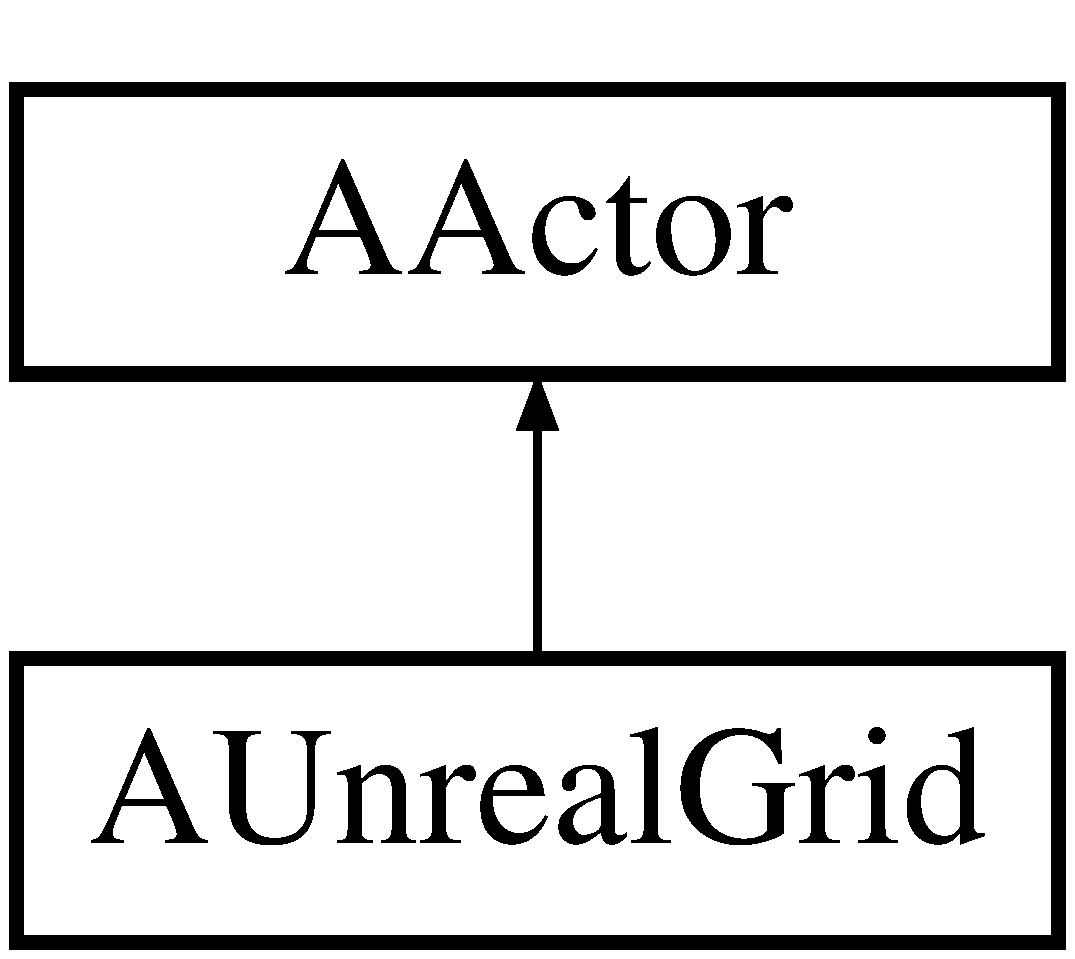
\includegraphics[height=2.000000cm]{class_a_unreal_grid}
\end{center}
\end{figure}
\subsection*{Public Member Functions}
\begin{DoxyCompactItemize}
\item 
virtual void \hyperlink{class_a_unreal_grid_a9f2e41aff1d7918e7bf46a93432ced89}{Begin\+Play} () override
\begin{DoxyCompactList}\small\item\em An inherited member. \end{DoxyCompactList}\item 
void \hyperlink{class_a_unreal_grid_ac418fa2ea58ef9c00939f441ccdff8d4}{Square\+Activate} (uint32 x, uint32 y)
\begin{DoxyCompactList}\small\item\em A public member taking in two variable. \end{DoxyCompactList}\item 
void \hyperlink{class_a_unreal_grid_ab6dd0588dcf8892df18183d9eae54036}{Highlight} (uint32 x, uint32 y)
\begin{DoxyCompactList}\small\item\em A public member taking in two variable. \end{DoxyCompactList}\item 
void \hyperlink{class_a_unreal_grid_a18fad8e1af79ff004c54c0a05b171f01}{Dim} (uint32 x, uint32 y)
\begin{DoxyCompactList}\small\item\em A public member taking in two variable. \end{DoxyCompactList}\item 
void \hyperlink{class_a_unreal_grid_a4de19b986295141d8a1b31ef872a2f43}{Show\+Path} (T\+Array$<$ \hyperlink{class_grid_pathing_cell}{Grid\+Pathing\+Cell} $>$ path)
\begin{DoxyCompactList}\small\item\em A public member taking in a variable. \end{DoxyCompactList}\item 
void \hyperlink{class_a_unreal_grid_a7c1328560c61da12f8e515f149457999}{Set\+Max\+Step} (uint32 m\+Step)
\begin{DoxyCompactList}\small\item\em A public member taking in a variable. \end{DoxyCompactList}\item 
void \hyperlink{class_a_unreal_grid_a53493ad37970ddcdf437475740fa73ac}{Clear\+Highlight} ()
\begin{DoxyCompactList}\small\item\em A public member. \end{DoxyCompactList}\item 
F\+O\+R\+C\+E\+I\+N\+L\+I\+NE class U\+Scene\+Component $\ast$ \hyperlink{class_a_unreal_grid_adc32753015f3681249c9effd0babf72d}{Get\+Dummy\+Root} () const
\begin{DoxyCompactList}\small\item\em A public member. \end{DoxyCompactList}\item 
F\+O\+R\+C\+E\+I\+N\+L\+I\+NE class U\+Text\+Render\+Component $\ast$ \hyperlink{class_a_unreal_grid_a2b699473afc36a77c3719002ae37bd9d}{Get\+Score\+Text} () const
\begin{DoxyCompactList}\small\item\em A public member. \end{DoxyCompactList}\end{DoxyCompactItemize}
\subsection*{Public Attributes}
\begin{DoxyCompactItemize}
\item 
bool \hyperlink{class_a_unreal_grid_a3c7f942498aac5d56e594f4c71be239b}{active\+Square}
\begin{DoxyCompactList}\small\item\em A public variable. \end{DoxyCompactList}\item 
int32 \hyperlink{class_a_unreal_grid_ab968c97a7b73c4c4a78752810340db86}{activeX}
\begin{DoxyCompactList}\small\item\em A public variable. \end{DoxyCompactList}\item 
int32 \hyperlink{class_a_unreal_grid_a112aaee76dadd64d889a14d1fc25cb2a}{activeY}
\begin{DoxyCompactList}\small\item\em A public variable. \end{DoxyCompactList}\item 
uint32 \hyperlink{class_a_unreal_grid_a17290d30345faf244ad5fabde26046ac}{max\+Step}
\begin{DoxyCompactList}\small\item\em A public variable. \end{DoxyCompactList}\item 
T\+Array$<$ \hyperlink{class_a_grid_block}{A\+Grid\+Block} $\ast$ $>$ \hyperlink{class_a_unreal_grid_a190e16b669bb5cb44c29765ba772c3f5}{cells}
\begin{DoxyCompactList}\small\item\em A public variable. \end{DoxyCompactList}\item 
int32 \hyperlink{class_a_unreal_grid_aff61595921013715b51b18bbd5d624ea}{Length}
\begin{DoxyCompactList}\small\item\em A public variable. \end{DoxyCompactList}\item 
int32 \hyperlink{class_a_unreal_grid_a7674836c06f6c4022f98bdecd72cb89c}{Height}
\begin{DoxyCompactList}\small\item\em A public variable. \end{DoxyCompactList}\item 
float \hyperlink{class_a_unreal_grid_ab7f6c7b674ee42393ddad1a070e94ead}{Block\+Spacing}
\begin{DoxyCompactList}\small\item\em A public variable. \end{DoxyCompactList}\item 
class \hyperlink{class_grid}{Grid} $\ast$ \hyperlink{class_a_unreal_grid_a1bc505d6a6df9d8d57db4d92bf7a0636}{Grid\+Model}
\begin{DoxyCompactList}\small\item\em A public variable. \end{DoxyCompactList}\item 
class \hyperlink{class_grid_pathing}{Grid\+Pathing} $\ast$ \hyperlink{class_a_unreal_grid_a5a108c220c0bfded8c7312aabbbcba82}{Grid\+Path}
\begin{DoxyCompactList}\small\item\em A public variable. \end{DoxyCompactList}\end{DoxyCompactItemize}


\subsection{Detailed Description}
Class for the grid, interfacing with Unreal. 

\subsection{Member Function Documentation}
\hypertarget{class_a_unreal_grid_a9f2e41aff1d7918e7bf46a93432ced89}{}\label{class_a_unreal_grid_a9f2e41aff1d7918e7bf46a93432ced89} 
\index{A\+Unreal\+Grid@{A\+Unreal\+Grid}!Begin\+Play@{Begin\+Play}}
\index{Begin\+Play@{Begin\+Play}!A\+Unreal\+Grid@{A\+Unreal\+Grid}}
\subsubsection{\texorpdfstring{Begin\+Play()}{BeginPlay()}}
{\footnotesize\ttfamily void A\+Unreal\+Grid\+::\+Begin\+Play (\begin{DoxyParamCaption}{ }\end{DoxyParamCaption})\hspace{0.3cm}{\ttfamily [override]}, {\ttfamily [virtual]}}



An inherited member. 

Begin A\+Actor Interface. \hypertarget{class_a_unreal_grid_a53493ad37970ddcdf437475740fa73ac}{}\label{class_a_unreal_grid_a53493ad37970ddcdf437475740fa73ac} 
\index{A\+Unreal\+Grid@{A\+Unreal\+Grid}!Clear\+Highlight@{Clear\+Highlight}}
\index{Clear\+Highlight@{Clear\+Highlight}!A\+Unreal\+Grid@{A\+Unreal\+Grid}}
\subsubsection{\texorpdfstring{Clear\+Highlight()}{ClearHighlight()}}
{\footnotesize\ttfamily void A\+Unreal\+Grid\+::\+Clear\+Highlight (\begin{DoxyParamCaption}{ }\end{DoxyParamCaption})}



A public member. 

Clears all highlights. \hypertarget{class_a_unreal_grid_a18fad8e1af79ff004c54c0a05b171f01}{}\label{class_a_unreal_grid_a18fad8e1af79ff004c54c0a05b171f01} 
\index{A\+Unreal\+Grid@{A\+Unreal\+Grid}!Dim@{Dim}}
\index{Dim@{Dim}!A\+Unreal\+Grid@{A\+Unreal\+Grid}}
\subsubsection{\texorpdfstring{Dim()}{Dim()}}
{\footnotesize\ttfamily void A\+Unreal\+Grid\+::\+Dim (\begin{DoxyParamCaption}\item[{uint32}]{x,  }\item[{uint32}]{y }\end{DoxyParamCaption})}



A public member taking in two variable. 

/param x x coordinate of the cell block /param y y coordinate of the cell block Dims the block on the x y coordinate. \hypertarget{class_a_unreal_grid_adc32753015f3681249c9effd0babf72d}{}\label{class_a_unreal_grid_adc32753015f3681249c9effd0babf72d} 
\index{A\+Unreal\+Grid@{A\+Unreal\+Grid}!Get\+Dummy\+Root@{Get\+Dummy\+Root}}
\index{Get\+Dummy\+Root@{Get\+Dummy\+Root}!A\+Unreal\+Grid@{A\+Unreal\+Grid}}
\subsubsection{\texorpdfstring{Get\+Dummy\+Root()}{GetDummyRoot()}}
{\footnotesize\ttfamily F\+O\+R\+C\+E\+I\+N\+L\+I\+NE class U\+Scene\+Component$\ast$ A\+Unreal\+Grid\+::\+Get\+Dummy\+Root (\begin{DoxyParamCaption}{ }\end{DoxyParamCaption}) const\hspace{0.3cm}{\ttfamily [inline]}}



A public member. 

Returns Dummy\+Root subobject. \hypertarget{class_a_unreal_grid_a2b699473afc36a77c3719002ae37bd9d}{}\label{class_a_unreal_grid_a2b699473afc36a77c3719002ae37bd9d} 
\index{A\+Unreal\+Grid@{A\+Unreal\+Grid}!Get\+Score\+Text@{Get\+Score\+Text}}
\index{Get\+Score\+Text@{Get\+Score\+Text}!A\+Unreal\+Grid@{A\+Unreal\+Grid}}
\subsubsection{\texorpdfstring{Get\+Score\+Text()}{GetScoreText()}}
{\footnotesize\ttfamily F\+O\+R\+C\+E\+I\+N\+L\+I\+NE class U\+Text\+Render\+Component$\ast$ A\+Unreal\+Grid\+::\+Get\+Score\+Text (\begin{DoxyParamCaption}{ }\end{DoxyParamCaption}) const\hspace{0.3cm}{\ttfamily [inline]}}



A public member. 

Returns Score\+Text subobject. \hypertarget{class_a_unreal_grid_ab6dd0588dcf8892df18183d9eae54036}{}\label{class_a_unreal_grid_ab6dd0588dcf8892df18183d9eae54036} 
\index{A\+Unreal\+Grid@{A\+Unreal\+Grid}!Highlight@{Highlight}}
\index{Highlight@{Highlight}!A\+Unreal\+Grid@{A\+Unreal\+Grid}}
\subsubsection{\texorpdfstring{Highlight()}{Highlight()}}
{\footnotesize\ttfamily void A\+Unreal\+Grid\+::\+Highlight (\begin{DoxyParamCaption}\item[{uint32}]{x,  }\item[{uint32}]{y }\end{DoxyParamCaption})}



A public member taking in two variable. 

/param x x coordinate of the cell block /param y y coordinate of the cell block Hightlights the block on the x y coordinate. \hypertarget{class_a_unreal_grid_a7c1328560c61da12f8e515f149457999}{}\label{class_a_unreal_grid_a7c1328560c61da12f8e515f149457999} 
\index{A\+Unreal\+Grid@{A\+Unreal\+Grid}!Set\+Max\+Step@{Set\+Max\+Step}}
\index{Set\+Max\+Step@{Set\+Max\+Step}!A\+Unreal\+Grid@{A\+Unreal\+Grid}}
\subsubsection{\texorpdfstring{Set\+Max\+Step()}{SetMaxStep()}}
{\footnotesize\ttfamily void A\+Unreal\+Grid\+::\+Set\+Max\+Step (\begin{DoxyParamCaption}\item[{uint32}]{m\+Step }\end{DoxyParamCaption})}



A public member taking in a variable. 

/param m\+Step the number to set the max\+Step to Sets max\+Step variable. \hypertarget{class_a_unreal_grid_a4de19b986295141d8a1b31ef872a2f43}{}\label{class_a_unreal_grid_a4de19b986295141d8a1b31ef872a2f43} 
\index{A\+Unreal\+Grid@{A\+Unreal\+Grid}!Show\+Path@{Show\+Path}}
\index{Show\+Path@{Show\+Path}!A\+Unreal\+Grid@{A\+Unreal\+Grid}}
\subsubsection{\texorpdfstring{Show\+Path()}{ShowPath()}}
{\footnotesize\ttfamily void A\+Unreal\+Grid\+::\+Show\+Path (\begin{DoxyParamCaption}\item[{T\+Array$<$ \hyperlink{class_grid_pathing_cell}{Grid\+Pathing\+Cell} $>$}]{path }\end{DoxyParamCaption})}



A public member taking in a variable. 

/param path array that contains the path, in cells Highlights a Path. \hypertarget{class_a_unreal_grid_ac418fa2ea58ef9c00939f441ccdff8d4}{}\label{class_a_unreal_grid_ac418fa2ea58ef9c00939f441ccdff8d4} 
\index{A\+Unreal\+Grid@{A\+Unreal\+Grid}!Square\+Activate@{Square\+Activate}}
\index{Square\+Activate@{Square\+Activate}!A\+Unreal\+Grid@{A\+Unreal\+Grid}}
\subsubsection{\texorpdfstring{Square\+Activate()}{SquareActivate()}}
{\footnotesize\ttfamily void A\+Unreal\+Grid\+::\+Square\+Activate (\begin{DoxyParamCaption}\item[{uint32}]{x,  }\item[{uint32}]{y }\end{DoxyParamCaption})}



A public member taking in two variable. 

/param x x coordinate of the cell block /param y y coordinate of the cell block Handles the block being clicked. 

\subsection{Member Data Documentation}
\hypertarget{class_a_unreal_grid_a3c7f942498aac5d56e594f4c71be239b}{}\label{class_a_unreal_grid_a3c7f942498aac5d56e594f4c71be239b} 
\index{A\+Unreal\+Grid@{A\+Unreal\+Grid}!active\+Square@{active\+Square}}
\index{active\+Square@{active\+Square}!A\+Unreal\+Grid@{A\+Unreal\+Grid}}
\subsubsection{\texorpdfstring{active\+Square}{activeSquare}}
{\footnotesize\ttfamily bool A\+Unreal\+Grid\+::active\+Square}



A public variable. 

has a square been selected \hypertarget{class_a_unreal_grid_ab968c97a7b73c4c4a78752810340db86}{}\label{class_a_unreal_grid_ab968c97a7b73c4c4a78752810340db86} 
\index{A\+Unreal\+Grid@{A\+Unreal\+Grid}!activeX@{activeX}}
\index{activeX@{activeX}!A\+Unreal\+Grid@{A\+Unreal\+Grid}}
\subsubsection{\texorpdfstring{activeX}{activeX}}
{\footnotesize\ttfamily int32 A\+Unreal\+Grid\+::activeX}



A public variable. 

Active\+Square x coordinate. \hypertarget{class_a_unreal_grid_a112aaee76dadd64d889a14d1fc25cb2a}{}\label{class_a_unreal_grid_a112aaee76dadd64d889a14d1fc25cb2a} 
\index{A\+Unreal\+Grid@{A\+Unreal\+Grid}!activeY@{activeY}}
\index{activeY@{activeY}!A\+Unreal\+Grid@{A\+Unreal\+Grid}}
\subsubsection{\texorpdfstring{activeY}{activeY}}
{\footnotesize\ttfamily int32 A\+Unreal\+Grid\+::activeY}



A public variable. 

Active\+Square y coordinate. \hypertarget{class_a_unreal_grid_ab7f6c7b674ee42393ddad1a070e94ead}{}\label{class_a_unreal_grid_ab7f6c7b674ee42393ddad1a070e94ead} 
\index{A\+Unreal\+Grid@{A\+Unreal\+Grid}!Block\+Spacing@{Block\+Spacing}}
\index{Block\+Spacing@{Block\+Spacing}!A\+Unreal\+Grid@{A\+Unreal\+Grid}}
\subsubsection{\texorpdfstring{Block\+Spacing}{BlockSpacing}}
{\footnotesize\ttfamily float A\+Unreal\+Grid\+::\+Block\+Spacing}



A public variable. 

Spacing of blocks. \hypertarget{class_a_unreal_grid_a190e16b669bb5cb44c29765ba772c3f5}{}\label{class_a_unreal_grid_a190e16b669bb5cb44c29765ba772c3f5} 
\index{A\+Unreal\+Grid@{A\+Unreal\+Grid}!cells@{cells}}
\index{cells@{cells}!A\+Unreal\+Grid@{A\+Unreal\+Grid}}
\subsubsection{\texorpdfstring{cells}{cells}}
{\footnotesize\ttfamily T\+Array$<$\hyperlink{class_a_grid_block}{A\+Grid\+Block}$\ast$$>$ A\+Unreal\+Grid\+::cells}



A public variable. 

T\+Array containing all Grid\+Blocks. \hypertarget{class_a_unreal_grid_a1bc505d6a6df9d8d57db4d92bf7a0636}{}\label{class_a_unreal_grid_a1bc505d6a6df9d8d57db4d92bf7a0636} 
\index{A\+Unreal\+Grid@{A\+Unreal\+Grid}!Grid\+Model@{Grid\+Model}}
\index{Grid\+Model@{Grid\+Model}!A\+Unreal\+Grid@{A\+Unreal\+Grid}}
\subsubsection{\texorpdfstring{Grid\+Model}{GridModel}}
{\footnotesize\ttfamily class \hyperlink{class_grid}{Grid}$\ast$ A\+Unreal\+Grid\+::\+Grid\+Model}



A public variable. 

Model grid. \hypertarget{class_a_unreal_grid_a5a108c220c0bfded8c7312aabbbcba82}{}\label{class_a_unreal_grid_a5a108c220c0bfded8c7312aabbbcba82} 
\index{A\+Unreal\+Grid@{A\+Unreal\+Grid}!Grid\+Path@{Grid\+Path}}
\index{Grid\+Path@{Grid\+Path}!A\+Unreal\+Grid@{A\+Unreal\+Grid}}
\subsubsection{\texorpdfstring{Grid\+Path}{GridPath}}
{\footnotesize\ttfamily class \hyperlink{class_grid_pathing}{Grid\+Pathing}$\ast$ A\+Unreal\+Grid\+::\+Grid\+Path}



A public variable. 

Pathing \hyperlink{class_grid}{Grid}. \hypertarget{class_a_unreal_grid_a7674836c06f6c4022f98bdecd72cb89c}{}\label{class_a_unreal_grid_a7674836c06f6c4022f98bdecd72cb89c} 
\index{A\+Unreal\+Grid@{A\+Unreal\+Grid}!Height@{Height}}
\index{Height@{Height}!A\+Unreal\+Grid@{A\+Unreal\+Grid}}
\subsubsection{\texorpdfstring{Height}{Height}}
{\footnotesize\ttfamily int32 A\+Unreal\+Grid\+::\+Height}



A public variable. 

Number of blocks along height of grid \hypertarget{class_a_unreal_grid_aff61595921013715b51b18bbd5d624ea}{}\label{class_a_unreal_grid_aff61595921013715b51b18bbd5d624ea} 
\index{A\+Unreal\+Grid@{A\+Unreal\+Grid}!Length@{Length}}
\index{Length@{Length}!A\+Unreal\+Grid@{A\+Unreal\+Grid}}
\subsubsection{\texorpdfstring{Length}{Length}}
{\footnotesize\ttfamily int32 A\+Unreal\+Grid\+::\+Length}



A public variable. 

Number of blocks along length of grid. \hypertarget{class_a_unreal_grid_a17290d30345faf244ad5fabde26046ac}{}\label{class_a_unreal_grid_a17290d30345faf244ad5fabde26046ac} 
\index{A\+Unreal\+Grid@{A\+Unreal\+Grid}!max\+Step@{max\+Step}}
\index{max\+Step@{max\+Step}!A\+Unreal\+Grid@{A\+Unreal\+Grid}}
\subsubsection{\texorpdfstring{max\+Step}{maxStep}}
{\footnotesize\ttfamily uint32 A\+Unreal\+Grid\+::max\+Step}



A public variable. 

Maximum number of steps that can be taken. 

The documentation for this class was generated from the following files\+:\begin{DoxyCompactItemize}
\item 
Unreal\+Grid.\+h\item 
Unreal\+Grid.\+cpp\end{DoxyCompactItemize}

\hypertarget{class_a_x_a3_character}{}\section{A\+X\+A3\+Character Class Reference}
\label{class_a_x_a3_character}\index{A\+X\+A3\+Character@{A\+X\+A3\+Character}}
Inheritance diagram for A\+X\+A3\+Character\+:\begin{figure}[H]
\begin{center}
\leavevmode
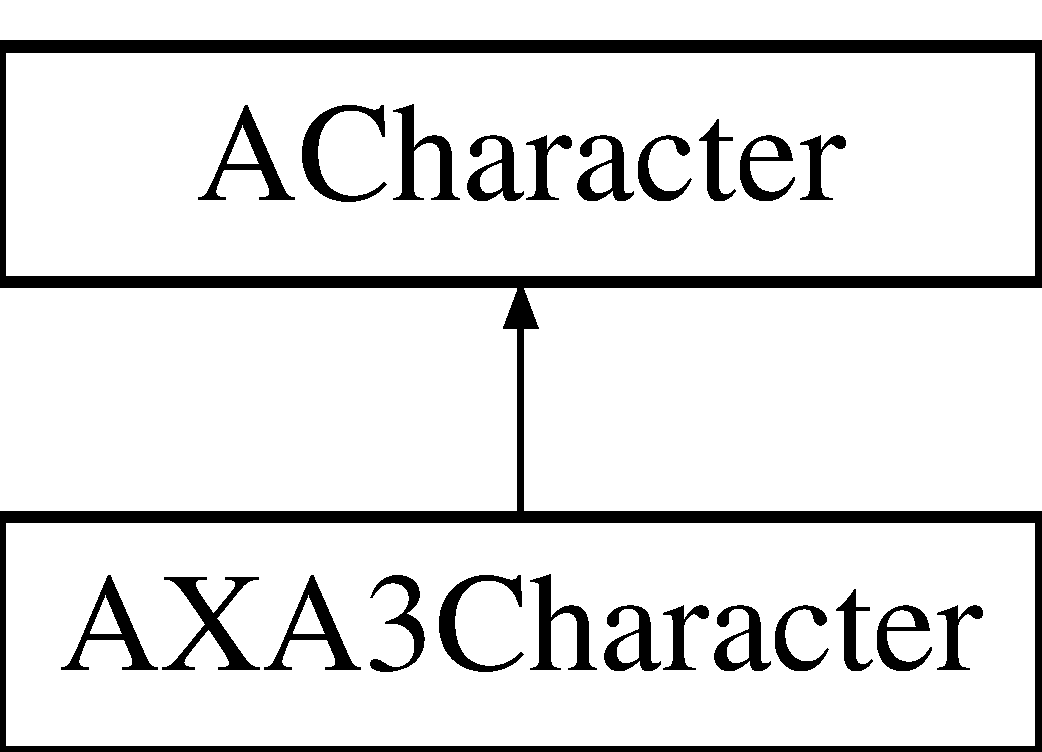
\includegraphics[height=2.000000cm]{class_a_x_a3_character}
\end{center}
\end{figure}
\subsection*{Public Member Functions}
\begin{DoxyCompactItemize}
\item 
\hypertarget{class_a_x_a3_character_ae2250498d9229d83448ddd91c05470d1}{}\label{class_a_x_a3_character_ae2250498d9229d83448ddd91c05470d1} 
virtual void {\bfseries Tick} (float Delta\+Seconds) override
\item 
F\+O\+R\+C\+E\+I\+N\+L\+I\+NE class U\+Camera\+Component $\ast$ \hyperlink{class_a_x_a3_character_a89f06b20e3c4350a374a821345bf424c}{Get\+Top\+Down\+Camera\+Component} () const
\item 
F\+O\+R\+C\+E\+I\+N\+L\+I\+NE class U\+Spring\+Arm\+Component $\ast$ \hyperlink{class_a_x_a3_character_ab8949643f5090f747b9882d8c7640748}{Get\+Camera\+Boom} () const
\item 
F\+O\+R\+C\+E\+I\+N\+L\+I\+NE class U\+Decal\+Component $\ast$ \hyperlink{class_a_x_a3_character_aea6ee1ad712275c59026b4c7b7b8edf2}{Get\+Cursor\+To\+World} ()
\end{DoxyCompactItemize}


\subsection{Member Function Documentation}
\hypertarget{class_a_x_a3_character_ab8949643f5090f747b9882d8c7640748}{}\label{class_a_x_a3_character_ab8949643f5090f747b9882d8c7640748} 
\index{A\+X\+A3\+Character@{A\+X\+A3\+Character}!Get\+Camera\+Boom@{Get\+Camera\+Boom}}
\index{Get\+Camera\+Boom@{Get\+Camera\+Boom}!A\+X\+A3\+Character@{A\+X\+A3\+Character}}
\subsubsection{\texorpdfstring{Get\+Camera\+Boom()}{GetCameraBoom()}}
{\footnotesize\ttfamily F\+O\+R\+C\+E\+I\+N\+L\+I\+NE class U\+Spring\+Arm\+Component$\ast$ A\+X\+A3\+Character\+::\+Get\+Camera\+Boom (\begin{DoxyParamCaption}{ }\end{DoxyParamCaption}) const\hspace{0.3cm}{\ttfamily [inline]}}

Returns Camera\+Boom subobject \hypertarget{class_a_x_a3_character_aea6ee1ad712275c59026b4c7b7b8edf2}{}\label{class_a_x_a3_character_aea6ee1ad712275c59026b4c7b7b8edf2} 
\index{A\+X\+A3\+Character@{A\+X\+A3\+Character}!Get\+Cursor\+To\+World@{Get\+Cursor\+To\+World}}
\index{Get\+Cursor\+To\+World@{Get\+Cursor\+To\+World}!A\+X\+A3\+Character@{A\+X\+A3\+Character}}
\subsubsection{\texorpdfstring{Get\+Cursor\+To\+World()}{GetCursorToWorld()}}
{\footnotesize\ttfamily F\+O\+R\+C\+E\+I\+N\+L\+I\+NE class U\+Decal\+Component$\ast$ A\+X\+A3\+Character\+::\+Get\+Cursor\+To\+World (\begin{DoxyParamCaption}{ }\end{DoxyParamCaption})\hspace{0.3cm}{\ttfamily [inline]}}

Returns Cursor\+To\+World subobject \hypertarget{class_a_x_a3_character_a89f06b20e3c4350a374a821345bf424c}{}\label{class_a_x_a3_character_a89f06b20e3c4350a374a821345bf424c} 
\index{A\+X\+A3\+Character@{A\+X\+A3\+Character}!Get\+Top\+Down\+Camera\+Component@{Get\+Top\+Down\+Camera\+Component}}
\index{Get\+Top\+Down\+Camera\+Component@{Get\+Top\+Down\+Camera\+Component}!A\+X\+A3\+Character@{A\+X\+A3\+Character}}
\subsubsection{\texorpdfstring{Get\+Top\+Down\+Camera\+Component()}{GetTopDownCameraComponent()}}
{\footnotesize\ttfamily F\+O\+R\+C\+E\+I\+N\+L\+I\+NE class U\+Camera\+Component$\ast$ A\+X\+A3\+Character\+::\+Get\+Top\+Down\+Camera\+Component (\begin{DoxyParamCaption}{ }\end{DoxyParamCaption}) const\hspace{0.3cm}{\ttfamily [inline]}}

Returns Top\+Down\+Camera\+Component subobject 

The documentation for this class was generated from the following files\+:\begin{DoxyCompactItemize}
\item 
X\+A3\+Character.\+h\item 
X\+A3\+Character.\+cpp\end{DoxyCompactItemize}

\hypertarget{class_a_x_a3_game_mode}{}\section{A\+X\+A3\+Game\+Mode Class Reference}
\label{class_a_x_a3_game_mode}\index{A\+X\+A3\+Game\+Mode@{A\+X\+A3\+Game\+Mode}}


Class for the Game Mode.  




{\ttfamily \#include $<$X\+A3\+Game\+Mode.\+h$>$}

Inheritance diagram for A\+X\+A3\+Game\+Mode\+:\begin{figure}[H]
\begin{center}
\leavevmode
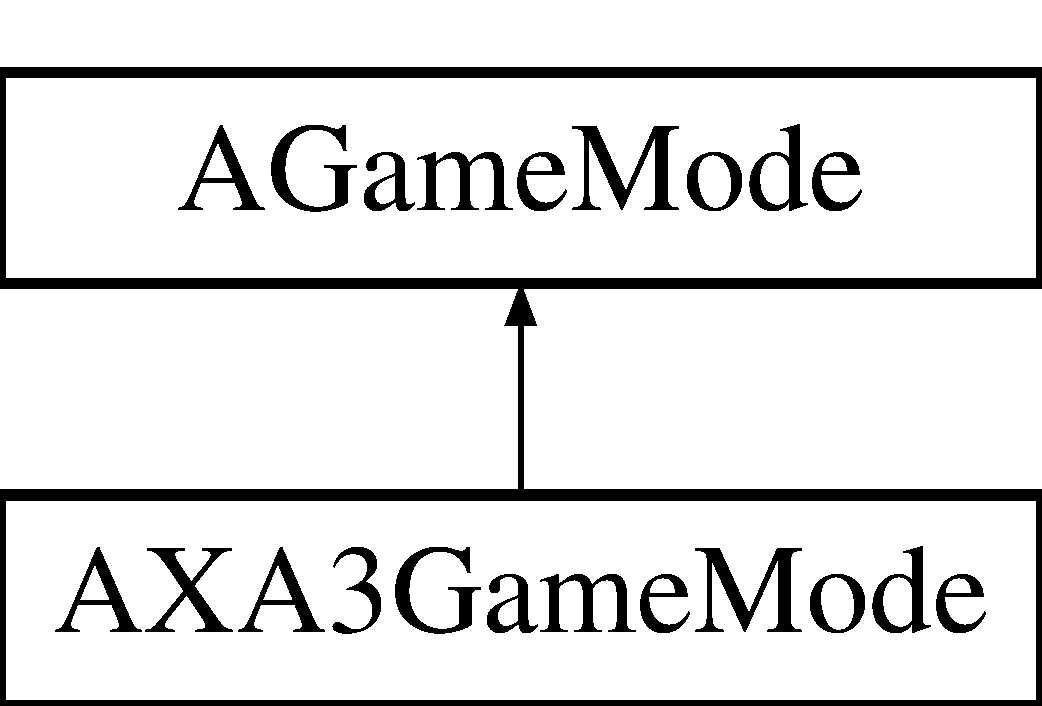
\includegraphics[height=2.000000cm]{class_a_x_a3_game_mode}
\end{center}
\end{figure}
\subsection*{Public Member Functions}
\begin{DoxyCompactItemize}
\item 
void \hyperlink{class_a_x_a3_game_mode_a5b84f33f7978a2015a870a6daab2ee68}{switch\+Sides} ()
\begin{DoxyCompactList}\small\item\em A public member. \end{DoxyCompactList}\item 
bool \hyperlink{class_a_x_a3_game_mode_a0a00cfd9dc6792556a48235fe9b7b151}{check\+End} ()
\begin{DoxyCompactList}\small\item\em A public member returning a boolean. \end{DoxyCompactList}\end{DoxyCompactItemize}
\subsection*{Protected Attributes}
\begin{DoxyCompactItemize}
\item 
bool \hyperlink{class_a_x_a3_game_mode_ab240472b5b7ebecb719d972ae3ad1167}{is\+Player\+One} = true
\begin{DoxyCompactList}\small\item\em A public variable. \end{DoxyCompactList}\end{DoxyCompactItemize}


\subsection{Detailed Description}
Class for the Game Mode. 

A class defining the basic game rules 

\subsection{Member Function Documentation}
\hypertarget{class_a_x_a3_game_mode_a0a00cfd9dc6792556a48235fe9b7b151}{}\label{class_a_x_a3_game_mode_a0a00cfd9dc6792556a48235fe9b7b151} 
\index{A\+X\+A3\+Game\+Mode@{A\+X\+A3\+Game\+Mode}!check\+End@{check\+End}}
\index{check\+End@{check\+End}!A\+X\+A3\+Game\+Mode@{A\+X\+A3\+Game\+Mode}}
\subsubsection{\texorpdfstring{check\+End()}{checkEnd()}}
{\footnotesize\ttfamily bool A\+X\+A3\+Game\+Mode\+::check\+End (\begin{DoxyParamCaption}{ }\end{DoxyParamCaption})}



A public member returning a boolean. 

Check if all Tu has been exhausted, returns boolean \hypertarget{class_a_x_a3_game_mode_a5b84f33f7978a2015a870a6daab2ee68}{}\label{class_a_x_a3_game_mode_a5b84f33f7978a2015a870a6daab2ee68} 
\index{A\+X\+A3\+Game\+Mode@{A\+X\+A3\+Game\+Mode}!switch\+Sides@{switch\+Sides}}
\index{switch\+Sides@{switch\+Sides}!A\+X\+A3\+Game\+Mode@{A\+X\+A3\+Game\+Mode}}
\subsubsection{\texorpdfstring{switch\+Sides()}{switchSides()}}
{\footnotesize\ttfamily void A\+X\+A3\+Game\+Mode\+::switch\+Sides (\begin{DoxyParamCaption}{ }\end{DoxyParamCaption})}



A public member. 

Switch the Current turn 

\subsection{Member Data Documentation}
\hypertarget{class_a_x_a3_game_mode_ab240472b5b7ebecb719d972ae3ad1167}{}\label{class_a_x_a3_game_mode_ab240472b5b7ebecb719d972ae3ad1167} 
\index{A\+X\+A3\+Game\+Mode@{A\+X\+A3\+Game\+Mode}!is\+Player\+One@{is\+Player\+One}}
\index{is\+Player\+One@{is\+Player\+One}!A\+X\+A3\+Game\+Mode@{A\+X\+A3\+Game\+Mode}}
\subsubsection{\texorpdfstring{is\+Player\+One}{isPlayerOne}}
{\footnotesize\ttfamily bool A\+X\+A3\+Game\+Mode\+::is\+Player\+One = true\hspace{0.3cm}{\ttfamily [protected]}}



A public variable. 

Is the current side one?A public variable.

Is the current side one? 

The documentation for this class was generated from the following files\+:\begin{DoxyCompactItemize}
\item 
X\+A3\+Game\+Mode.\+h\item 
X\+A3\+Game\+Mode.\+cpp\end{DoxyCompactItemize}

\hypertarget{class_a_x_a3_player_controller}{}\section{A\+X\+A3\+Player\+Controller Class Reference}
\label{class_a_x_a3_player_controller}\index{A\+X\+A3\+Player\+Controller@{A\+X\+A3\+Player\+Controller}}


Class for the Controller.  




{\ttfamily \#include $<$X\+A3\+Player\+Controller.\+h$>$}

Inheritance diagram for A\+X\+A3\+Player\+Controller\+:\begin{figure}[H]
\begin{center}
\leavevmode
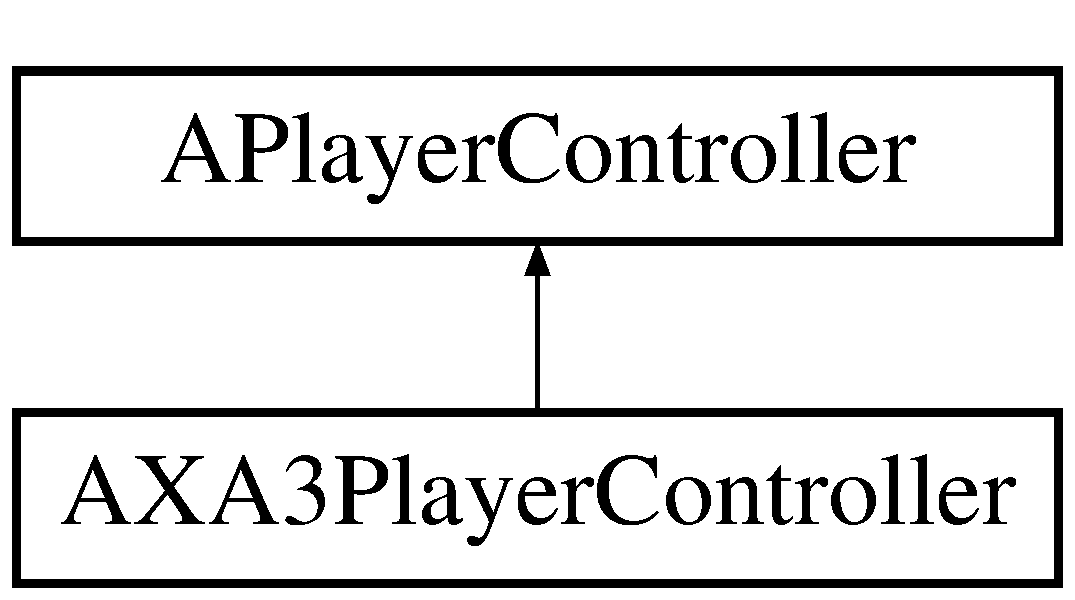
\includegraphics[height=2.000000cm]{class_a_x_a3_player_controller}
\end{center}
\end{figure}
\subsection*{Public Member Functions}
\begin{DoxyCompactItemize}
\item 
void \hyperlink{class_a_x_a3_player_controller_aa419797ca4c60bb27a033a307c5ccbee}{Set\+New\+Move\+Destination} (const F\+Vector Dest\+Location)
\begin{DoxyCompactList}\small\item\em Normal Member taking a constand F\+Vector. \end{DoxyCompactList}\item 
void \hyperlink{class_a_x_a3_player_controller_ab559e4393ede764953acd4c868a41eef}{On\+Set\+Destination\+Pressed} ()
\begin{DoxyCompactList}\small\item\em Normal Member. \end{DoxyCompactList}\item 
void \hyperlink{class_a_x_a3_player_controller_a08d57685ee2b9f7f4d347707113f77c1}{On\+Set\+Destination\+Released} ()
\begin{DoxyCompactList}\small\item\em Normal Member. \end{DoxyCompactList}\end{DoxyCompactItemize}
\subsection*{Protected Member Functions}
\begin{DoxyCompactItemize}
\item 
virtual void \hyperlink{class_a_x_a3_player_controller_a4517394eaa773561191813ea4c2959b6}{Player\+Tick} (float Delta\+Time) override
\begin{DoxyCompactList}\small\item\em Inherited Member taking in a float. \end{DoxyCompactList}\item 
virtual void \hyperlink{class_a_x_a3_player_controller_ae1a9e48d7cb021a81ea0357b3be6afa6}{Setup\+Input\+Component} () override
\begin{DoxyCompactList}\small\item\em Inherited Member. \end{DoxyCompactList}\item 
void \hyperlink{class_a_x_a3_player_controller_a799e0ef8edbdb796c7b5286a7e53bac6}{On\+Reset\+VR} ()
\item 
void \hyperlink{class_a_x_a3_player_controller_a14779b01d600fdb7b9f4440e06e8288d}{Move\+To\+Mouse\+Cursor} ()
\begin{DoxyCompactList}\small\item\em Normal Member. \end{DoxyCompactList}\item 
void \hyperlink{class_a_x_a3_player_controller_a491c620eeaa2db69f8fb4e5a2b1c5cb3}{Move\+To\+Touch\+Location} (const E\+Touch\+Index\+::\+Type Finger\+Index, const F\+Vector Location)
\begin{DoxyCompactList}\small\item\em Normal Member. \end{DoxyCompactList}\end{DoxyCompactItemize}
\subsection*{Protected Attributes}
\begin{DoxyCompactItemize}
\item 
uint32 \hyperlink{class_a_x_a3_player_controller_af4d6c8b0909b0bc00e5b1df2437353bb}{b\+Move\+To\+Mouse\+Cursor}\+: 1
\begin{DoxyCompactList}\small\item\em A protected variable. \end{DoxyCompactList}\end{DoxyCompactItemize}


\subsection{Detailed Description}
Class for the Controller. 

A class that contains relevant functions to controll the play character. 

\subsection{Member Function Documentation}
\hypertarget{class_a_x_a3_player_controller_a14779b01d600fdb7b9f4440e06e8288d}{}\label{class_a_x_a3_player_controller_a14779b01d600fdb7b9f4440e06e8288d} 
\index{A\+X\+A3\+Player\+Controller@{A\+X\+A3\+Player\+Controller}!Move\+To\+Mouse\+Cursor@{Move\+To\+Mouse\+Cursor}}
\index{Move\+To\+Mouse\+Cursor@{Move\+To\+Mouse\+Cursor}!A\+X\+A3\+Player\+Controller@{A\+X\+A3\+Player\+Controller}}
\subsubsection{\texorpdfstring{Move\+To\+Mouse\+Cursor()}{MoveToMouseCursor()}}
{\footnotesize\ttfamily void A\+X\+A3\+Player\+Controller\+::\+Move\+To\+Mouse\+Cursor (\begin{DoxyParamCaption}{ }\end{DoxyParamCaption})\hspace{0.3cm}{\ttfamily [protected]}}



Normal Member. 

Navigate player to the current mouse cursor location. \hypertarget{class_a_x_a3_player_controller_a491c620eeaa2db69f8fb4e5a2b1c5cb3}{}\label{class_a_x_a3_player_controller_a491c620eeaa2db69f8fb4e5a2b1c5cb3} 
\index{A\+X\+A3\+Player\+Controller@{A\+X\+A3\+Player\+Controller}!Move\+To\+Touch\+Location@{Move\+To\+Touch\+Location}}
\index{Move\+To\+Touch\+Location@{Move\+To\+Touch\+Location}!A\+X\+A3\+Player\+Controller@{A\+X\+A3\+Player\+Controller}}
\subsubsection{\texorpdfstring{Move\+To\+Touch\+Location()}{MoveToTouchLocation()}}
{\footnotesize\ttfamily void A\+X\+A3\+Player\+Controller\+::\+Move\+To\+Touch\+Location (\begin{DoxyParamCaption}\item[{const E\+Touch\+Index\+::\+Type}]{Finger\+Index,  }\item[{const F\+Vector}]{Location }\end{DoxyParamCaption})\hspace{0.3cm}{\ttfamily [protected]}}



Normal Member. 

Navigate player to the current touch location. \hypertarget{class_a_x_a3_player_controller_a799e0ef8edbdb796c7b5286a7e53bac6}{}\label{class_a_x_a3_player_controller_a799e0ef8edbdb796c7b5286a7e53bac6} 
\index{A\+X\+A3\+Player\+Controller@{A\+X\+A3\+Player\+Controller}!On\+Reset\+VR@{On\+Reset\+VR}}
\index{On\+Reset\+VR@{On\+Reset\+VR}!A\+X\+A3\+Player\+Controller@{A\+X\+A3\+Player\+Controller}}
\subsubsection{\texorpdfstring{On\+Reset\+V\+R()}{OnResetVR()}}
{\footnotesize\ttfamily void A\+X\+A3\+Player\+Controller\+::\+On\+Reset\+VR (\begin{DoxyParamCaption}{ }\end{DoxyParamCaption})\hspace{0.3cm}{\ttfamily [protected]}}

Resets H\+MD orientation in VR. \hypertarget{class_a_x_a3_player_controller_ab559e4393ede764953acd4c868a41eef}{}\label{class_a_x_a3_player_controller_ab559e4393ede764953acd4c868a41eef} 
\index{A\+X\+A3\+Player\+Controller@{A\+X\+A3\+Player\+Controller}!On\+Set\+Destination\+Pressed@{On\+Set\+Destination\+Pressed}}
\index{On\+Set\+Destination\+Pressed@{On\+Set\+Destination\+Pressed}!A\+X\+A3\+Player\+Controller@{A\+X\+A3\+Player\+Controller}}
\subsubsection{\texorpdfstring{On\+Set\+Destination\+Pressed()}{OnSetDestinationPressed()}}
{\footnotesize\ttfamily void A\+X\+A3\+Player\+Controller\+::\+On\+Set\+Destination\+Pressed (\begin{DoxyParamCaption}{ }\end{DoxyParamCaption})}



Normal Member. 

Input handlers for Set\+Destination action. \hypertarget{class_a_x_a3_player_controller_a08d57685ee2b9f7f4d347707113f77c1}{}\label{class_a_x_a3_player_controller_a08d57685ee2b9f7f4d347707113f77c1} 
\index{A\+X\+A3\+Player\+Controller@{A\+X\+A3\+Player\+Controller}!On\+Set\+Destination\+Released@{On\+Set\+Destination\+Released}}
\index{On\+Set\+Destination\+Released@{On\+Set\+Destination\+Released}!A\+X\+A3\+Player\+Controller@{A\+X\+A3\+Player\+Controller}}
\subsubsection{\texorpdfstring{On\+Set\+Destination\+Released()}{OnSetDestinationReleased()}}
{\footnotesize\ttfamily void A\+X\+A3\+Player\+Controller\+::\+On\+Set\+Destination\+Released (\begin{DoxyParamCaption}{ }\end{DoxyParamCaption})}



Normal Member. 

Input handlers for Set\+Destination action. \hypertarget{class_a_x_a3_player_controller_a4517394eaa773561191813ea4c2959b6}{}\label{class_a_x_a3_player_controller_a4517394eaa773561191813ea4c2959b6} 
\index{A\+X\+A3\+Player\+Controller@{A\+X\+A3\+Player\+Controller}!Player\+Tick@{Player\+Tick}}
\index{Player\+Tick@{Player\+Tick}!A\+X\+A3\+Player\+Controller@{A\+X\+A3\+Player\+Controller}}
\subsubsection{\texorpdfstring{Player\+Tick()}{PlayerTick()}}
{\footnotesize\ttfamily void A\+X\+A3\+Player\+Controller\+::\+Player\+Tick (\begin{DoxyParamCaption}\item[{float}]{Delta\+Time }\end{DoxyParamCaption})\hspace{0.3cm}{\ttfamily [override]}, {\ttfamily [protected]}, {\ttfamily [virtual]}}



Inherited Member taking in a float. 

Tick method for refresh. \hypertarget{class_a_x_a3_player_controller_aa419797ca4c60bb27a033a307c5ccbee}{}\label{class_a_x_a3_player_controller_aa419797ca4c60bb27a033a307c5ccbee} 
\index{A\+X\+A3\+Player\+Controller@{A\+X\+A3\+Player\+Controller}!Set\+New\+Move\+Destination@{Set\+New\+Move\+Destination}}
\index{Set\+New\+Move\+Destination@{Set\+New\+Move\+Destination}!A\+X\+A3\+Player\+Controller@{A\+X\+A3\+Player\+Controller}}
\subsubsection{\texorpdfstring{Set\+New\+Move\+Destination()}{SetNewMoveDestination()}}
{\footnotesize\ttfamily void A\+X\+A3\+Player\+Controller\+::\+Set\+New\+Move\+Destination (\begin{DoxyParamCaption}\item[{const F\+Vector}]{Dest\+Location }\end{DoxyParamCaption})}



Normal Member taking a constand F\+Vector. 

/param Dest\+Location vector for destination Navigate player to the given world location. \hypertarget{class_a_x_a3_player_controller_ae1a9e48d7cb021a81ea0357b3be6afa6}{}\label{class_a_x_a3_player_controller_ae1a9e48d7cb021a81ea0357b3be6afa6} 
\index{A\+X\+A3\+Player\+Controller@{A\+X\+A3\+Player\+Controller}!Setup\+Input\+Component@{Setup\+Input\+Component}}
\index{Setup\+Input\+Component@{Setup\+Input\+Component}!A\+X\+A3\+Player\+Controller@{A\+X\+A3\+Player\+Controller}}
\subsubsection{\texorpdfstring{Setup\+Input\+Component()}{SetupInputComponent()}}
{\footnotesize\ttfamily void A\+X\+A3\+Player\+Controller\+::\+Setup\+Input\+Component (\begin{DoxyParamCaption}{ }\end{DoxyParamCaption})\hspace{0.3cm}{\ttfamily [override]}, {\ttfamily [protected]}, {\ttfamily [virtual]}}



Inherited Member. 

Set up inputs. 

\subsection{Member Data Documentation}
\hypertarget{class_a_x_a3_player_controller_af4d6c8b0909b0bc00e5b1df2437353bb}{}\label{class_a_x_a3_player_controller_af4d6c8b0909b0bc00e5b1df2437353bb} 
\index{A\+X\+A3\+Player\+Controller@{A\+X\+A3\+Player\+Controller}!b\+Move\+To\+Mouse\+Cursor@{b\+Move\+To\+Mouse\+Cursor}}
\index{b\+Move\+To\+Mouse\+Cursor@{b\+Move\+To\+Mouse\+Cursor}!A\+X\+A3\+Player\+Controller@{A\+X\+A3\+Player\+Controller}}
\subsubsection{\texorpdfstring{b\+Move\+To\+Mouse\+Cursor}{bMoveToMouseCursor}}
{\footnotesize\ttfamily uint32 A\+X\+A3\+Player\+Controller\+::b\+Move\+To\+Mouse\+Cursor\hspace{0.3cm}{\ttfamily [protected]}}



A protected variable. 

boolean for whether the controlled character should navigate to the mouse cursor. 

The documentation for this class was generated from the following files\+:\begin{DoxyCompactItemize}
\item 
X\+A3\+Player\+Controller.\+h\item 
X\+A3\+Player\+Controller.\+cpp\end{DoxyCompactItemize}

\hypertarget{class_grid}{}\section{Grid Class Reference}
\label{class_grid}\index{Grid@{Grid}}


Class for the \hyperlink{class_grid}{Grid}.  




{\ttfamily \#include $<$Grid.\+h$>$}

\subsection*{Public Member Functions}
\begin{DoxyCompactItemize}
\item 
\hyperlink{class_grid_a3602235a1d7b17254b0219dc7b754456}{Grid} (uint16 iH, uint16 iW)
\begin{DoxyCompactList}\small\item\em Constructor taking in two unsigned integer values. \end{DoxyCompactList}\item 
\hyperlink{class_grid_a5c60d994d3dcfab965bf7b62d028a797}{Grid} (uint16 Tarr\mbox{[}$\,$\mbox{]})
\begin{DoxyCompactList}\small\item\em Constructor taking in two unsigned integer values. \end{DoxyCompactList}\item 
uint16 \hyperlink{class_grid_a165ea0d0c65632335dbe7df2bc34a030}{get\+Terrain} (uint16 ix, uint16 iy)
\begin{DoxyCompactList}\small\item\em Public member taking in two variables and returning an unsigned integer value. \end{DoxyCompactList}\item 
void \hyperlink{class_grid_a3feb00999e05825bbb470bdc098e05ab}{set\+Terrain} (uint16 ix, uint16 iy, uint16 i\+Terrain)
\begin{DoxyCompactList}\small\item\em Public member taking in three variables. \end{DoxyCompactList}\item 
void \hyperlink{class_grid_a4704642a117a8be8e9defdda92784303}{set\+Properties} (uint16 ix, uint16 iy, uint16 i\+Terrain, bool b\+Blocking, bool b\+Occupied)
\begin{DoxyCompactList}\small\item\em Public member taking in five variables. \end{DoxyCompactList}\item 
bool \hyperlink{class_grid_afbfece3a3d96fa4e40316ad9cdf61c98}{is\+Occupied} (uint16 ix, uint16 iy)
\begin{DoxyCompactList}\small\item\em Public member taking in two variables and returning a boolean value. \end{DoxyCompactList}\item 
void \hyperlink{class_grid_a4142f2281cbb882c39514ffc3c2a59af}{set\+Occupied} (uint16 ix, uint16 iy, bool b\+Occupied)
\begin{DoxyCompactList}\small\item\em Public member taking in three variables. \end{DoxyCompactList}\item 
void \hyperlink{class_grid_af15e440bc92017e805740db43a09c034}{move} (uint16 i\+OldX, uint16 i\+OldY, uint16 i\+NewX, uint16 i\+NewY)
\begin{DoxyCompactList}\small\item\em Public member takeing in four variables. \end{DoxyCompactList}\item 
bool \hyperlink{class_grid_a8f12a73036cc2f155e20030dfae6b6f6}{is\+Blocked} (uint16 ix, uint16 iy)
\begin{DoxyCompactList}\small\item\em Public member taking in two variables and returning a boolean value. \end{DoxyCompactList}\item 
void \hyperlink{class_grid_a19e1e00ddf325821bc0c16de9f7799ed}{set\+Blocked} (uint16 ix, uint16 iy, bool b\+Blocked)
\begin{DoxyCompactList}\small\item\em Public member taking in three variables. \end{DoxyCompactList}\item 
uint16 \hyperlink{class_grid_ab03502a2a92f1890e5e453e5878c66db}{get\+Width} ()
\begin{DoxyCompactList}\small\item\em Public member returning an unsigned int. \end{DoxyCompactList}\item 
uint16 \hyperlink{class_grid_a374615638fd9e5f587d28486295952ef}{get\+Height} ()
\begin{DoxyCompactList}\small\item\em Public member returning an unsigned int. \end{DoxyCompactList}\end{DoxyCompactItemize}


\subsection{Detailed Description}
Class for the \hyperlink{class_grid}{Grid}. 

\hyperlink{class_grid}{Grid} class that contains infromation on terrain, current occupation, and other properties 

\subsection{Constructor \& Destructor Documentation}
\hypertarget{class_grid_a3602235a1d7b17254b0219dc7b754456}{}\label{class_grid_a3602235a1d7b17254b0219dc7b754456} 
\index{Grid@{Grid}!Grid@{Grid}}
\index{Grid@{Grid}!Grid@{Grid}}
\subsubsection{\texorpdfstring{Grid()}{Grid()}\hspace{0.1cm}{\footnotesize\ttfamily [1/2]}}
{\footnotesize\ttfamily Grid\+::\+Grid (\begin{DoxyParamCaption}\item[{uint16}]{iH,  }\item[{uint16}]{iW }\end{DoxyParamCaption})}



Constructor taking in two unsigned integer values. 

/param iH Height of the \hyperlink{class_grid}{Grid} /param iW Width of the grid Initiate the object with Height and Width values. \hypertarget{class_grid_a5c60d994d3dcfab965bf7b62d028a797}{}\label{class_grid_a5c60d994d3dcfab965bf7b62d028a797} 
\index{Grid@{Grid}!Grid@{Grid}}
\index{Grid@{Grid}!Grid@{Grid}}
\subsubsection{\texorpdfstring{Grid()}{Grid()}\hspace{0.1cm}{\footnotesize\ttfamily [2/2]}}
{\footnotesize\ttfamily Grid\+::\+Grid (\begin{DoxyParamCaption}\item[{uint16}]{Tarr\mbox{[}$\,$\mbox{]} }\end{DoxyParamCaption})}



Constructor taking in two unsigned integer values. 

/param Tarr width and height of the grid in an array Initiate the object with Height and Width values. 

\subsection{Member Function Documentation}
\hypertarget{class_grid_a374615638fd9e5f587d28486295952ef}{}\label{class_grid_a374615638fd9e5f587d28486295952ef} 
\index{Grid@{Grid}!get\+Height@{get\+Height}}
\index{get\+Height@{get\+Height}!Grid@{Grid}}
\subsubsection{\texorpdfstring{get\+Height()}{getHeight()}}
{\footnotesize\ttfamily uint16 Grid\+::get\+Height (\begin{DoxyParamCaption}{ }\end{DoxyParamCaption})}



Public member returning an unsigned int. 

Get the Height of the grid. \hypertarget{class_grid_a165ea0d0c65632335dbe7df2bc34a030}{}\label{class_grid_a165ea0d0c65632335dbe7df2bc34a030} 
\index{Grid@{Grid}!get\+Terrain@{get\+Terrain}}
\index{get\+Terrain@{get\+Terrain}!Grid@{Grid}}
\subsubsection{\texorpdfstring{get\+Terrain()}{getTerrain()}}
{\footnotesize\ttfamily uint16 Grid\+::get\+Terrain (\begin{DoxyParamCaption}\item[{uint16}]{ix,  }\item[{uint16}]{iy }\end{DoxyParamCaption})}



Public member taking in two variables and returning an unsigned integer value. 

/param ix x coordinate of the cell /param iy y coordinate of the cell Get the terrain value of the cell pertaining to the x and y coordinate. \hypertarget{class_grid_ab03502a2a92f1890e5e453e5878c66db}{}\label{class_grid_ab03502a2a92f1890e5e453e5878c66db} 
\index{Grid@{Grid}!get\+Width@{get\+Width}}
\index{get\+Width@{get\+Width}!Grid@{Grid}}
\subsubsection{\texorpdfstring{get\+Width()}{getWidth()}}
{\footnotesize\ttfamily uint16 Grid\+::get\+Width (\begin{DoxyParamCaption}{ }\end{DoxyParamCaption})}



Public member returning an unsigned int. 

Get the Width of the grid. \hypertarget{class_grid_a8f12a73036cc2f155e20030dfae6b6f6}{}\label{class_grid_a8f12a73036cc2f155e20030dfae6b6f6} 
\index{Grid@{Grid}!is\+Blocked@{is\+Blocked}}
\index{is\+Blocked@{is\+Blocked}!Grid@{Grid}}
\subsubsection{\texorpdfstring{is\+Blocked()}{isBlocked()}}
{\footnotesize\ttfamily bool Grid\+::is\+Blocked (\begin{DoxyParamCaption}\item[{uint16}]{ix,  }\item[{uint16}]{iy }\end{DoxyParamCaption})}



Public member taking in two variables and returning a boolean value. 

/param ix x coordinate of the cell /param iy y coordinate of the cell Get if the cell at the x and y coordinate is blocked. \hypertarget{class_grid_afbfece3a3d96fa4e40316ad9cdf61c98}{}\label{class_grid_afbfece3a3d96fa4e40316ad9cdf61c98} 
\index{Grid@{Grid}!is\+Occupied@{is\+Occupied}}
\index{is\+Occupied@{is\+Occupied}!Grid@{Grid}}
\subsubsection{\texorpdfstring{is\+Occupied()}{isOccupied()}}
{\footnotesize\ttfamily bool Grid\+::is\+Occupied (\begin{DoxyParamCaption}\item[{uint16}]{ix,  }\item[{uint16}]{iy }\end{DoxyParamCaption})}



Public member taking in two variables and returning a boolean value. 

/param ix x coordinate of the cell /param iy y coordinate of the cell Get if the cell at the x and y coordinate is occupied. \hypertarget{class_grid_af15e440bc92017e805740db43a09c034}{}\label{class_grid_af15e440bc92017e805740db43a09c034} 
\index{Grid@{Grid}!move@{move}}
\index{move@{move}!Grid@{Grid}}
\subsubsection{\texorpdfstring{move()}{move()}}
{\footnotesize\ttfamily void Grid\+::move (\begin{DoxyParamCaption}\item[{uint16}]{i\+OldX,  }\item[{uint16}]{i\+OldY,  }\item[{uint16}]{i\+NewX,  }\item[{uint16}]{i\+NewY }\end{DoxyParamCaption})}



Public member takeing in four variables. 

/param i\+Oldx x coordinate of the old cell /param i\+Oldy y coordinate of the old cell /param i\+Newx x coordinate of the new cell /param i\+Newy y coordinate of the new cell Move something from one cell to another. \hypertarget{class_grid_a19e1e00ddf325821bc0c16de9f7799ed}{}\label{class_grid_a19e1e00ddf325821bc0c16de9f7799ed} 
\index{Grid@{Grid}!set\+Blocked@{set\+Blocked}}
\index{set\+Blocked@{set\+Blocked}!Grid@{Grid}}
\subsubsection{\texorpdfstring{set\+Blocked()}{setBlocked()}}
{\footnotesize\ttfamily void Grid\+::set\+Blocked (\begin{DoxyParamCaption}\item[{uint16}]{ix,  }\item[{uint16}]{iy,  }\item[{bool}]{b\+Blocked }\end{DoxyParamCaption})}



Public member taking in three variables. 

/param ix x coordinate of the cell /param iy y coordinate of the cell /param b\+Blocked boolean for if the cell is Blocked Set the b\+Blocked vallue at x and y. \hypertarget{class_grid_a4142f2281cbb882c39514ffc3c2a59af}{}\label{class_grid_a4142f2281cbb882c39514ffc3c2a59af} 
\index{Grid@{Grid}!set\+Occupied@{set\+Occupied}}
\index{set\+Occupied@{set\+Occupied}!Grid@{Grid}}
\subsubsection{\texorpdfstring{set\+Occupied()}{setOccupied()}}
{\footnotesize\ttfamily void Grid\+::set\+Occupied (\begin{DoxyParamCaption}\item[{uint16}]{ix,  }\item[{uint16}]{iy,  }\item[{bool}]{b\+Occupied }\end{DoxyParamCaption})}



Public member taking in three variables. 

/param ix x coordinate of the cell /param iy y coordinate of the cell /param b\+Occupied boolean for if the cell is occupied Set the b\+Occupied vallue at x and y. \hypertarget{class_grid_a4704642a117a8be8e9defdda92784303}{}\label{class_grid_a4704642a117a8be8e9defdda92784303} 
\index{Grid@{Grid}!set\+Properties@{set\+Properties}}
\index{set\+Properties@{set\+Properties}!Grid@{Grid}}
\subsubsection{\texorpdfstring{set\+Properties()}{setProperties()}}
{\footnotesize\ttfamily void Grid\+::set\+Properties (\begin{DoxyParamCaption}\item[{uint16}]{ix,  }\item[{uint16}]{iy,  }\item[{uint16}]{i\+Terrain,  }\item[{bool}]{b\+Blocking,  }\item[{bool}]{b\+Occupied }\end{DoxyParamCaption})}



Public member taking in five variables. 

/param ix x coordinate of the cell /param iy y coordinate of the cell /param i\+Terrain terrain value of the cell /param b\+Blocking boolean for if the cell is blocking movement /param b\+Occupied boolean for if the cell is occupied Set the properties of the grid cell \hypertarget{class_grid_a3feb00999e05825bbb470bdc098e05ab}{}\label{class_grid_a3feb00999e05825bbb470bdc098e05ab} 
\index{Grid@{Grid}!set\+Terrain@{set\+Terrain}}
\index{set\+Terrain@{set\+Terrain}!Grid@{Grid}}
\subsubsection{\texorpdfstring{set\+Terrain()}{setTerrain()}}
{\footnotesize\ttfamily void Grid\+::set\+Terrain (\begin{DoxyParamCaption}\item[{uint16}]{ix,  }\item[{uint16}]{iy,  }\item[{uint16}]{i\+Terrain }\end{DoxyParamCaption})}



Public member taking in three variables. 

/param ix x coordinate of the cell /param iy y coordinate of the cell /param i\+Terrain terrain value of the cell Set the terrain value of the cell pertaining to the x and y coordinate. 

The documentation for this class was generated from the following files\+:\begin{DoxyCompactItemize}
\item 
Grid.\+h\item 
Grid.\+cpp\end{DoxyCompactItemize}

\hypertarget{class_grid_pathing}{}\section{Grid\+Pathing Class Reference}
\label{class_grid_pathing}\index{Grid\+Pathing@{Grid\+Pathing}}


Class for Pathing Units on the \hyperlink{class_grid}{Grid}.  




{\ttfamily \#include $<$Grid\+Pathing.\+h$>$}

\subsection*{Public Member Functions}
\begin{DoxyCompactItemize}
\item 
\hypertarget{class_grid_pathing_a015d8d2d2181c40a11fa2403c47834a8}{}\label{class_grid_pathing_a015d8d2d2181c40a11fa2403c47834a8} 
{\bfseries Grid\+Pathing} (T\+Shared\+Ptr$<$ \hyperlink{class_grid}{Grid} $>$ g)
\item 
T\+Array$<$ \hyperlink{class_grid_pathing_cell}{Grid\+Pathing\+Cell} $>$ \hyperlink{class_grid_pathing_a34564759aeef0f39b6c596163530b51b}{path\+To} (uint16 x\+Init, uint16 y\+Init, uint16 x\+Final, uint16 y\+Final, uint16 max\+Step)
\begin{DoxyCompactList}\small\item\em A public member taking in five variables returning a \hyperlink{class_grid_pathing_cell}{Grid\+Pathing\+Cell} Array. \end{DoxyCompactList}\item 
void \hyperlink{class_grid_pathing_a0d4652be2afba5e6363af1459a8720d2}{explorer} (uint16 x, uint16 y, uint16 score, uint16 max\+Step)
\begin{DoxyCompactList}\small\item\em A public member taking in four variables. \end{DoxyCompactList}\item 
uint16 \hyperlink{class_grid_pathing_aa7d6f9ce481bf8148d778419dfc5947b}{calc\+Index} (uint16 x, uint16 y)
\begin{DoxyCompactList}\small\item\em A public member taking in two variables and returning a variable. \end{DoxyCompactList}\item 
bool \hyperlink{class_grid_pathing_a97cdae33476da7638fbcd45fc0595eb9}{is\+Valid\+Next\+Cell} (uint16 x, uint16 y, uint16 score, uint16 max\+Step)
\begin{DoxyCompactList}\small\item\em A public member taking in four variables and returning a boolean value. \end{DoxyCompactList}\item 
void \hyperlink{class_grid_pathing_a1cad627b7af6d693e2b6fbabae4a54cc}{synthesis} (uint16 x\+Init, uint16 y\+Init, uint16 x\+Final, uint16 y\+Final)
\begin{DoxyCompactList}\small\item\em A public member taking in four variables. \end{DoxyCompactList}\item 
void \hyperlink{class_grid_pathing_aa4ce89d949c8d42bf2d4eb9d77e865a8}{reset} ()
\begin{DoxyCompactList}\small\item\em A public member. \end{DoxyCompactList}\item 
bool \hyperlink{class_grid_pathing_a037817191233010bfb337e78142583b3}{is\+Pathable} (uint16 x, uint16 y)
\begin{DoxyCompactList}\small\item\em A public member taking in two variables and returning a boolean value. \end{DoxyCompactList}\end{DoxyCompactItemize}
\subsection*{Public Attributes}
\begin{DoxyCompactItemize}
\item 
T\+Array$<$ \hyperlink{class_grid_pathing_cell}{Grid\+Pathing\+Cell} $>$ \hyperlink{class_grid_pathing_a5f136ffddfd481828d8e3bd4bd68c469}{final\+Path}
\begin{DoxyCompactList}\small\item\em A public array variable. \end{DoxyCompactList}\item 
T\+Shared\+Ptr$<$ \hyperlink{class_grid}{Grid} $>$ \hyperlink{class_grid_pathing_a7dd028322c2248c079d5c9aff06389e3}{grid}
\begin{DoxyCompactList}\small\item\em A public Pointer Array. \end{DoxyCompactList}\item 
T\+Array$<$ \hyperlink{class_grid_pathing_cell}{Grid\+Pathing\+Cell} $>$ \hyperlink{class_grid_pathing_abe2319f19bada22c1a20e5ae544b1ed2}{pathing\+Array}
\begin{DoxyCompactList}\small\item\em A public Pointer Array. \end{DoxyCompactList}\end{DoxyCompactItemize}


\subsection{Detailed Description}
Class for Pathing Units on the \hyperlink{class_grid}{Grid}. 

A class that uses the \hyperlink{class_grid_pathing_cell}{Grid\+Pathing\+Cell} class to determine the closest path from one point on the grid to another. 

\subsection{Member Function Documentation}
\hypertarget{class_grid_pathing_aa7d6f9ce481bf8148d778419dfc5947b}{}\label{class_grid_pathing_aa7d6f9ce481bf8148d778419dfc5947b} 
\index{Grid\+Pathing@{Grid\+Pathing}!calc\+Index@{calc\+Index}}
\index{calc\+Index@{calc\+Index}!Grid\+Pathing@{Grid\+Pathing}}
\subsubsection{\texorpdfstring{calc\+Index()}{calcIndex()}}
{\footnotesize\ttfamily uint16 Grid\+Pathing\+::calc\+Index (\begin{DoxyParamCaption}\item[{uint16}]{x,  }\item[{uint16}]{y }\end{DoxyParamCaption})}



A public member taking in two variables and returning a variable. 

/param x x value of the cell /param y y value of the cell A method to calculate the index of the cell. \hypertarget{class_grid_pathing_a0d4652be2afba5e6363af1459a8720d2}{}\label{class_grid_pathing_a0d4652be2afba5e6363af1459a8720d2} 
\index{Grid\+Pathing@{Grid\+Pathing}!explorer@{explorer}}
\index{explorer@{explorer}!Grid\+Pathing@{Grid\+Pathing}}
\subsubsection{\texorpdfstring{explorer()}{explorer()}}
{\footnotesize\ttfamily void Grid\+Pathing\+::explorer (\begin{DoxyParamCaption}\item[{uint16}]{x,  }\item[{uint16}]{y,  }\item[{uint16}]{score,  }\item[{uint16}]{max\+Step }\end{DoxyParamCaption})}



A public member taking in four variables. 

/param x x value of the cell /param y y value of the cell /param score score of the path /param max\+Step the maximum number of steps any unit can take, to limit the number of cells the pathing algorithm will search for A method to recursively visits each cell of the grid in a certain path to score it and point the cells to the previous cell in the optimal path. \hypertarget{class_grid_pathing_a037817191233010bfb337e78142583b3}{}\label{class_grid_pathing_a037817191233010bfb337e78142583b3} 
\index{Grid\+Pathing@{Grid\+Pathing}!is\+Pathable@{is\+Pathable}}
\index{is\+Pathable@{is\+Pathable}!Grid\+Pathing@{Grid\+Pathing}}
\subsubsection{\texorpdfstring{is\+Pathable()}{isPathable()}}
{\footnotesize\ttfamily bool Grid\+Pathing\+::is\+Pathable (\begin{DoxyParamCaption}\item[{uint16}]{x,  }\item[{uint16}]{y }\end{DoxyParamCaption})}



A public member taking in two variables and returning a boolean value. 

/param x x value of the cell /param y y value of the cell A method to deterimine whether a path can be calculated based on the x and y location of the cell. \hypertarget{class_grid_pathing_a97cdae33476da7638fbcd45fc0595eb9}{}\label{class_grid_pathing_a97cdae33476da7638fbcd45fc0595eb9} 
\index{Grid\+Pathing@{Grid\+Pathing}!is\+Valid\+Next\+Cell@{is\+Valid\+Next\+Cell}}
\index{is\+Valid\+Next\+Cell@{is\+Valid\+Next\+Cell}!Grid\+Pathing@{Grid\+Pathing}}
\subsubsection{\texorpdfstring{is\+Valid\+Next\+Cell()}{isValidNextCell()}}
{\footnotesize\ttfamily bool Grid\+Pathing\+::is\+Valid\+Next\+Cell (\begin{DoxyParamCaption}\item[{uint16}]{x,  }\item[{uint16}]{y,  }\item[{uint16}]{score,  }\item[{uint16}]{max\+Step }\end{DoxyParamCaption})}



A public member taking in four variables and returning a boolean value. 

/param x x value of the cell /param y y value of the cell /param score score of the path /param max\+Step the maximum number of steps any unit can take, to limit the number of cells the pathing algorithm will search for A method to deterimine if the next cell is a valid one. \hypertarget{class_grid_pathing_a34564759aeef0f39b6c596163530b51b}{}\label{class_grid_pathing_a34564759aeef0f39b6c596163530b51b} 
\index{Grid\+Pathing@{Grid\+Pathing}!path\+To@{path\+To}}
\index{path\+To@{path\+To}!Grid\+Pathing@{Grid\+Pathing}}
\subsubsection{\texorpdfstring{path\+To()}{pathTo()}}
{\footnotesize\ttfamily T\+Array$<$ \hyperlink{class_grid_pathing_cell}{Grid\+Pathing\+Cell} $>$ Grid\+Pathing\+::path\+To (\begin{DoxyParamCaption}\item[{uint16}]{x\+Init,  }\item[{uint16}]{y\+Init,  }\item[{uint16}]{x\+Final,  }\item[{uint16}]{y\+Final,  }\item[{uint16}]{max\+Step }\end{DoxyParamCaption})}



A public member taking in five variables returning a \hyperlink{class_grid_pathing_cell}{Grid\+Pathing\+Cell} Array. 

/param x\+Init x value of the starting cell /param y\+Init y value of the starting cell /param x\+Final x value of the ending cell /param y\+Final y value of the ending cell /param max\+Step the maximum number of steps any unit can take, to limit the number of cells the pathing algorithm will search for Uses recursive methods to return the final path. \hypertarget{class_grid_pathing_aa4ce89d949c8d42bf2d4eb9d77e865a8}{}\label{class_grid_pathing_aa4ce89d949c8d42bf2d4eb9d77e865a8} 
\index{Grid\+Pathing@{Grid\+Pathing}!reset@{reset}}
\index{reset@{reset}!Grid\+Pathing@{Grid\+Pathing}}
\subsubsection{\texorpdfstring{reset()}{reset()}}
{\footnotesize\ttfamily void Grid\+Pathing\+::reset (\begin{DoxyParamCaption}{ }\end{DoxyParamCaption})}



A public member. 

A method to reset the pathing array \hypertarget{class_grid_pathing_a1cad627b7af6d693e2b6fbabae4a54cc}{}\label{class_grid_pathing_a1cad627b7af6d693e2b6fbabae4a54cc} 
\index{Grid\+Pathing@{Grid\+Pathing}!synthesis@{synthesis}}
\index{synthesis@{synthesis}!Grid\+Pathing@{Grid\+Pathing}}
\subsubsection{\texorpdfstring{synthesis()}{synthesis()}}
{\footnotesize\ttfamily void Grid\+Pathing\+::synthesis (\begin{DoxyParamCaption}\item[{uint16}]{x\+Init,  }\item[{uint16}]{y\+Init,  }\item[{uint16}]{x\+Final,  }\item[{uint16}]{y\+Final }\end{DoxyParamCaption})}



A public member taking in four variables. 

/param x\+Init x value of the starting cell /param y\+Init y value of the starting cell /param x\+Final x value of the ending cell /param y\+Final y value of the ending cell A method that takes the now filled matrix of scores and \char`\"{}connected nodes\char`\"{} (cell objects which has a valid lastX and lastY) and traces out a path from the origin to a certain destination cell. 

\subsection{Member Data Documentation}
\hypertarget{class_grid_pathing_a5f136ffddfd481828d8e3bd4bd68c469}{}\label{class_grid_pathing_a5f136ffddfd481828d8e3bd4bd68c469} 
\index{Grid\+Pathing@{Grid\+Pathing}!final\+Path@{final\+Path}}
\index{final\+Path@{final\+Path}!Grid\+Pathing@{Grid\+Pathing}}
\subsubsection{\texorpdfstring{final\+Path}{finalPath}}
{\footnotesize\ttfamily T\+Array$<$\hyperlink{class_grid_pathing_cell}{Grid\+Pathing\+Cell}$>$ Grid\+Pathing\+::final\+Path}



A public array variable. 

Array that contains cells that are in the final path between the two points. \hypertarget{class_grid_pathing_a7dd028322c2248c079d5c9aff06389e3}{}\label{class_grid_pathing_a7dd028322c2248c079d5c9aff06389e3} 
\index{Grid\+Pathing@{Grid\+Pathing}!grid@{grid}}
\index{grid@{grid}!Grid\+Pathing@{Grid\+Pathing}}
\subsubsection{\texorpdfstring{grid}{grid}}
{\footnotesize\ttfamily T\+Shared\+Ptr$<$\hyperlink{class_grid}{Grid}$>$ Grid\+Pathing\+::grid}



A public Pointer Array. 

The grid that pathing is done on. \hypertarget{class_grid_pathing_abe2319f19bada22c1a20e5ae544b1ed2}{}\label{class_grid_pathing_abe2319f19bada22c1a20e5ae544b1ed2} 
\index{Grid\+Pathing@{Grid\+Pathing}!pathing\+Array@{pathing\+Array}}
\index{pathing\+Array@{pathing\+Array}!Grid\+Pathing@{Grid\+Pathing}}
\subsubsection{\texorpdfstring{pathing\+Array}{pathingArray}}
{\footnotesize\ttfamily T\+Array$<$\hyperlink{class_grid_pathing_cell}{Grid\+Pathing\+Cell}$>$ Grid\+Pathing\+::pathing\+Array}



A public Pointer Array. 

The array of cells used to path. 

The documentation for this class was generated from the following files\+:\begin{DoxyCompactItemize}
\item 
Grid\+Pathing.\+h\item 
Grid\+Pathing.\+cpp\end{DoxyCompactItemize}

\hypertarget{class_grid_pathing_cell}{}\section{Grid\+Pathing\+Cell Class Reference}
\label{class_grid_pathing_cell}\index{Grid\+Pathing\+Cell@{Grid\+Pathing\+Cell}}


Class for Cells in the grid, required for pathin.  




{\ttfamily \#include $<$Grid\+Pathing\+Cell.\+h$>$}

\subsection*{Public Member Functions}
\begin{DoxyCompactItemize}
\item 
\hyperlink{class_grid_pathing_cell_acbe865cb1e21ae9e22fda91a6eac7a57}{Grid\+Pathing\+Cell} (uint16 x\+Cord, uint16 y\+Cord)
\begin{DoxyCompactList}\small\item\em Constructor taking in two unsigned integer values. \end{DoxyCompactList}\item 
void \hyperlink{class_grid_pathing_cell_a6d360533681a9fc827b0b01c12f9fbf1}{set\+Last} (uint16 x\+Cord, uint16 y\+Cord)
\begin{DoxyCompactList}\small\item\em A public member that takes in two variables. \end{DoxyCompactList}\item 
void \hyperlink{class_grid_pathing_cell_a7e0b53ba48d7aa0576147759836b933a}{set\+Score} (uint16 \hyperlink{class_grid_pathing_cell_ab4d6783c766e718c20b173a89fe8e74d}{score})
\begin{DoxyCompactList}\small\item\em A public member that takes in a variables. \end{DoxyCompactList}\item 
void \hyperlink{class_grid_pathing_cell_ae706bf7d75f31d2a00d5e6de28da635c}{reset} ()
\begin{DoxyCompactList}\small\item\em A public member. \end{DoxyCompactList}\item 
uint16 \hyperlink{class_grid_pathing_cell_afa21d615e383d1f01664590903d71f8f}{get\+Score} ()
\begin{DoxyCompactList}\small\item\em A public member returning an unsigned integer value. \end{DoxyCompactList}\item 
T\+Array$<$ int16 $>$ \hyperlink{class_grid_pathing_cell_ad188a53ba82a3ee991f57cc3fdd0fb5f}{get\+Last} ()
\begin{DoxyCompactList}\small\item\em A public member returning an integer array. \end{DoxyCompactList}\item 
uint16 \hyperlink{class_grid_pathing_cell_aa4d5642ce2427123298c94b49ba7967a}{getX} ()
\begin{DoxyCompactList}\small\item\em A public member returning an unsigned integer value. \end{DoxyCompactList}\item 
uint16 \hyperlink{class_grid_pathing_cell_af1690d5798fb128d6bbf850375402ce1}{getY} ()
\begin{DoxyCompactList}\small\item\em A public member returning an unsigned integer value. \end{DoxyCompactList}\item 
\hyperlink{class_grid_pathing_cell_ad249acb6a70659728d0b872a2978fd39}{Grid\+Pathing\+Cell} (const \hyperlink{class_grid_pathing_cell}{Grid\+Pathing\+Cell} \&origin)
\begin{DoxyCompactList}\small\item\em Constructor taking in a \hyperlink{class_grid_pathing_cell}{Grid\+Pathing\+Cell}. \end{DoxyCompactList}\end{DoxyCompactItemize}
\subsection*{Public Attributes}
\begin{DoxyCompactItemize}
\item 
uint16 \hyperlink{class_grid_pathing_cell_a489c6c82b1ba484e9f9145c00ec165c0}{x}
\begin{DoxyCompactList}\small\item\em A public variable. \end{DoxyCompactList}\item 
uint16 \hyperlink{class_grid_pathing_cell_a32de04e3614f2e37622a281fdbc24d66}{y}
\begin{DoxyCompactList}\small\item\em A public variable. \end{DoxyCompactList}\item 
uint16 \hyperlink{class_grid_pathing_cell_ab4d6783c766e718c20b173a89fe8e74d}{score}
\begin{DoxyCompactList}\small\item\em A public variable. \end{DoxyCompactList}\item 
int16 \hyperlink{class_grid_pathing_cell_a3b2f9ec49d3e8a2aa3588eda310c8029}{x\+Last}
\begin{DoxyCompactList}\small\item\em A public variable. \end{DoxyCompactList}\item 
int16 \hyperlink{class_grid_pathing_cell_a3a1c2724f3308954f52f77c09d7d6d62}{y\+Last}
\begin{DoxyCompactList}\small\item\em A public variable. \end{DoxyCompactList}\end{DoxyCompactItemize}


\subsection{Detailed Description}
Class for Cells in the grid, required for pathin. 

A class that contains perameters of the grid pathing cell, an object that represents individual cells in a grid. Used in the \hyperlink{class_grid_pathing}{Grid\+Pathing} class 

\subsection{Constructor \& Destructor Documentation}
\hypertarget{class_grid_pathing_cell_acbe865cb1e21ae9e22fda91a6eac7a57}{}\label{class_grid_pathing_cell_acbe865cb1e21ae9e22fda91a6eac7a57} 
\index{Grid\+Pathing\+Cell@{Grid\+Pathing\+Cell}!Grid\+Pathing\+Cell@{Grid\+Pathing\+Cell}}
\index{Grid\+Pathing\+Cell@{Grid\+Pathing\+Cell}!Grid\+Pathing\+Cell@{Grid\+Pathing\+Cell}}
\subsubsection{\texorpdfstring{Grid\+Pathing\+Cell()}{GridPathingCell()}\hspace{0.1cm}{\footnotesize\ttfamily [1/2]}}
{\footnotesize\ttfamily Grid\+Pathing\+Cell\+::\+Grid\+Pathing\+Cell (\begin{DoxyParamCaption}\item[{uint16}]{x\+Cord,  }\item[{uint16}]{y\+Cord }\end{DoxyParamCaption})}



Constructor taking in two unsigned integer values. 

/param x\+Cord x coordinate of the cell /param y\+Cord y coordinate of the cell Initiate the object with x and y coordinates. \hypertarget{class_grid_pathing_cell_ad249acb6a70659728d0b872a2978fd39}{}\label{class_grid_pathing_cell_ad249acb6a70659728d0b872a2978fd39} 
\index{Grid\+Pathing\+Cell@{Grid\+Pathing\+Cell}!Grid\+Pathing\+Cell@{Grid\+Pathing\+Cell}}
\index{Grid\+Pathing\+Cell@{Grid\+Pathing\+Cell}!Grid\+Pathing\+Cell@{Grid\+Pathing\+Cell}}
\subsubsection{\texorpdfstring{Grid\+Pathing\+Cell()}{GridPathingCell()}\hspace{0.1cm}{\footnotesize\ttfamily [2/2]}}
{\footnotesize\ttfamily Grid\+Pathing\+Cell\+::\+Grid\+Pathing\+Cell (\begin{DoxyParamCaption}\item[{const \hyperlink{class_grid_pathing_cell}{Grid\+Pathing\+Cell} \&}]{origin }\end{DoxyParamCaption})}



Constructor taking in a \hyperlink{class_grid_pathing_cell}{Grid\+Pathing\+Cell}. 

/param origin the origin cell \hyperlink{class_grid}{Grid} Pathing constructor with a \hyperlink{class_grid}{Grid} Pathing object. 

\subsection{Member Function Documentation}
\hypertarget{class_grid_pathing_cell_ad188a53ba82a3ee991f57cc3fdd0fb5f}{}\label{class_grid_pathing_cell_ad188a53ba82a3ee991f57cc3fdd0fb5f} 
\index{Grid\+Pathing\+Cell@{Grid\+Pathing\+Cell}!get\+Last@{get\+Last}}
\index{get\+Last@{get\+Last}!Grid\+Pathing\+Cell@{Grid\+Pathing\+Cell}}
\subsubsection{\texorpdfstring{get\+Last()}{getLast()}}
{\footnotesize\ttfamily T\+Array$<$ int16 $>$ Grid\+Pathing\+Cell\+::get\+Last (\begin{DoxyParamCaption}{ }\end{DoxyParamCaption})}



A public member returning an integer array. 

Get the x\+Last and y\+Last values as an array. \hypertarget{class_grid_pathing_cell_afa21d615e383d1f01664590903d71f8f}{}\label{class_grid_pathing_cell_afa21d615e383d1f01664590903d71f8f} 
\index{Grid\+Pathing\+Cell@{Grid\+Pathing\+Cell}!get\+Score@{get\+Score}}
\index{get\+Score@{get\+Score}!Grid\+Pathing\+Cell@{Grid\+Pathing\+Cell}}
\subsubsection{\texorpdfstring{get\+Score()}{getScore()}}
{\footnotesize\ttfamily uint16 Grid\+Pathing\+Cell\+::get\+Score (\begin{DoxyParamCaption}{ }\end{DoxyParamCaption})}



A public member returning an unsigned integer value. 

Get the score of the cell. \hypertarget{class_grid_pathing_cell_aa4d5642ce2427123298c94b49ba7967a}{}\label{class_grid_pathing_cell_aa4d5642ce2427123298c94b49ba7967a} 
\index{Grid\+Pathing\+Cell@{Grid\+Pathing\+Cell}!getX@{getX}}
\index{getX@{getX}!Grid\+Pathing\+Cell@{Grid\+Pathing\+Cell}}
\subsubsection{\texorpdfstring{get\+X()}{getX()}}
{\footnotesize\ttfamily uint16 Grid\+Pathing\+Cell\+::getX (\begin{DoxyParamCaption}{ }\end{DoxyParamCaption})}



A public member returning an unsigned integer value. 

Get X. \hypertarget{class_grid_pathing_cell_af1690d5798fb128d6bbf850375402ce1}{}\label{class_grid_pathing_cell_af1690d5798fb128d6bbf850375402ce1} 
\index{Grid\+Pathing\+Cell@{Grid\+Pathing\+Cell}!getY@{getY}}
\index{getY@{getY}!Grid\+Pathing\+Cell@{Grid\+Pathing\+Cell}}
\subsubsection{\texorpdfstring{get\+Y()}{getY()}}
{\footnotesize\ttfamily uint16 Grid\+Pathing\+Cell\+::getY (\begin{DoxyParamCaption}{ }\end{DoxyParamCaption})}



A public member returning an unsigned integer value. 

Get Y. \hypertarget{class_grid_pathing_cell_ae706bf7d75f31d2a00d5e6de28da635c}{}\label{class_grid_pathing_cell_ae706bf7d75f31d2a00d5e6de28da635c} 
\index{Grid\+Pathing\+Cell@{Grid\+Pathing\+Cell}!reset@{reset}}
\index{reset@{reset}!Grid\+Pathing\+Cell@{Grid\+Pathing\+Cell}}
\subsubsection{\texorpdfstring{reset()}{reset()}}
{\footnotesize\ttfamily void Grid\+Pathing\+Cell\+::reset (\begin{DoxyParamCaption}{ }\end{DoxyParamCaption})}



A public member. 

Reset the cell. \hypertarget{class_grid_pathing_cell_a6d360533681a9fc827b0b01c12f9fbf1}{}\label{class_grid_pathing_cell_a6d360533681a9fc827b0b01c12f9fbf1} 
\index{Grid\+Pathing\+Cell@{Grid\+Pathing\+Cell}!set\+Last@{set\+Last}}
\index{set\+Last@{set\+Last}!Grid\+Pathing\+Cell@{Grid\+Pathing\+Cell}}
\subsubsection{\texorpdfstring{set\+Last()}{setLast()}}
{\footnotesize\ttfamily void Grid\+Pathing\+Cell\+::set\+Last (\begin{DoxyParamCaption}\item[{uint16}]{x\+Cord,  }\item[{uint16}]{y\+Cord }\end{DoxyParamCaption})}



A public member that takes in two variables. 

/param x\+Cord x value to set x\+Last to /param y\+Cord y value to set y\+Last to Set the last X Y coordinates of the cell. \hypertarget{class_grid_pathing_cell_a7e0b53ba48d7aa0576147759836b933a}{}\label{class_grid_pathing_cell_a7e0b53ba48d7aa0576147759836b933a} 
\index{Grid\+Pathing\+Cell@{Grid\+Pathing\+Cell}!set\+Score@{set\+Score}}
\index{set\+Score@{set\+Score}!Grid\+Pathing\+Cell@{Grid\+Pathing\+Cell}}
\subsubsection{\texorpdfstring{set\+Score()}{setScore()}}
{\footnotesize\ttfamily void Grid\+Pathing\+Cell\+::set\+Score (\begin{DoxyParamCaption}\item[{uint16}]{score }\end{DoxyParamCaption})}



A public member that takes in a variables. 

/param score score to be set to Set score of the cell. 

\subsection{Member Data Documentation}
\hypertarget{class_grid_pathing_cell_ab4d6783c766e718c20b173a89fe8e74d}{}\label{class_grid_pathing_cell_ab4d6783c766e718c20b173a89fe8e74d} 
\index{Grid\+Pathing\+Cell@{Grid\+Pathing\+Cell}!score@{score}}
\index{score@{score}!Grid\+Pathing\+Cell@{Grid\+Pathing\+Cell}}
\subsubsection{\texorpdfstring{score}{score}}
{\footnotesize\ttfamily uint16 Grid\+Pathing\+Cell\+::score}



A public variable. 

Cost of reaching this cell from the origin, with diagonals worth more than horizontals and verticals \hypertarget{class_grid_pathing_cell_a489c6c82b1ba484e9f9145c00ec165c0}{}\label{class_grid_pathing_cell_a489c6c82b1ba484e9f9145c00ec165c0} 
\index{Grid\+Pathing\+Cell@{Grid\+Pathing\+Cell}!x@{x}}
\index{x@{x}!Grid\+Pathing\+Cell@{Grid\+Pathing\+Cell}}
\subsubsection{\texorpdfstring{x}{x}}
{\footnotesize\ttfamily uint16 Grid\+Pathing\+Cell\+::x}



A public variable. 

X coordinate of the cell. \hypertarget{class_grid_pathing_cell_a3b2f9ec49d3e8a2aa3588eda310c8029}{}\label{class_grid_pathing_cell_a3b2f9ec49d3e8a2aa3588eda310c8029} 
\index{Grid\+Pathing\+Cell@{Grid\+Pathing\+Cell}!x\+Last@{x\+Last}}
\index{x\+Last@{x\+Last}!Grid\+Pathing\+Cell@{Grid\+Pathing\+Cell}}
\subsubsection{\texorpdfstring{x\+Last}{xLast}}
{\footnotesize\ttfamily int16 Grid\+Pathing\+Cell\+::x\+Last}



A public variable. 

X coordinate of the last cell to reach this one from the origin with the lowest score. \hypertarget{class_grid_pathing_cell_a32de04e3614f2e37622a281fdbc24d66}{}\label{class_grid_pathing_cell_a32de04e3614f2e37622a281fdbc24d66} 
\index{Grid\+Pathing\+Cell@{Grid\+Pathing\+Cell}!y@{y}}
\index{y@{y}!Grid\+Pathing\+Cell@{Grid\+Pathing\+Cell}}
\subsubsection{\texorpdfstring{y}{y}}
{\footnotesize\ttfamily uint16 Grid\+Pathing\+Cell\+::y}



A public variable. 

Y coordinate of the cell. \hypertarget{class_grid_pathing_cell_a3a1c2724f3308954f52f77c09d7d6d62}{}\label{class_grid_pathing_cell_a3a1c2724f3308954f52f77c09d7d6d62} 
\index{Grid\+Pathing\+Cell@{Grid\+Pathing\+Cell}!y\+Last@{y\+Last}}
\index{y\+Last@{y\+Last}!Grid\+Pathing\+Cell@{Grid\+Pathing\+Cell}}
\subsubsection{\texorpdfstring{y\+Last}{yLast}}
{\footnotesize\ttfamily int16 Grid\+Pathing\+Cell\+::y\+Last}



A public variable. 

Y coordinate of the last cell to reach this one from the origin with the lowest score. 

The documentation for this class was generated from the following files\+:\begin{DoxyCompactItemize}
\item 
Grid\+Pathing\+Cell.\+h\item 
Grid\+Pathing\+Cell.\+cpp\end{DoxyCompactItemize}

\hypertarget{class_u_context_menu}{}\section{U\+Context\+Menu Class Reference}
\label{class_u_context_menu}\index{U\+Context\+Menu@{U\+Context\+Menu}}


Class for UI.  




{\ttfamily \#include $<$Context\+Menu.\+h$>$}

Inheritance diagram for U\+Context\+Menu\+:\begin{figure}[H]
\begin{center}
\leavevmode
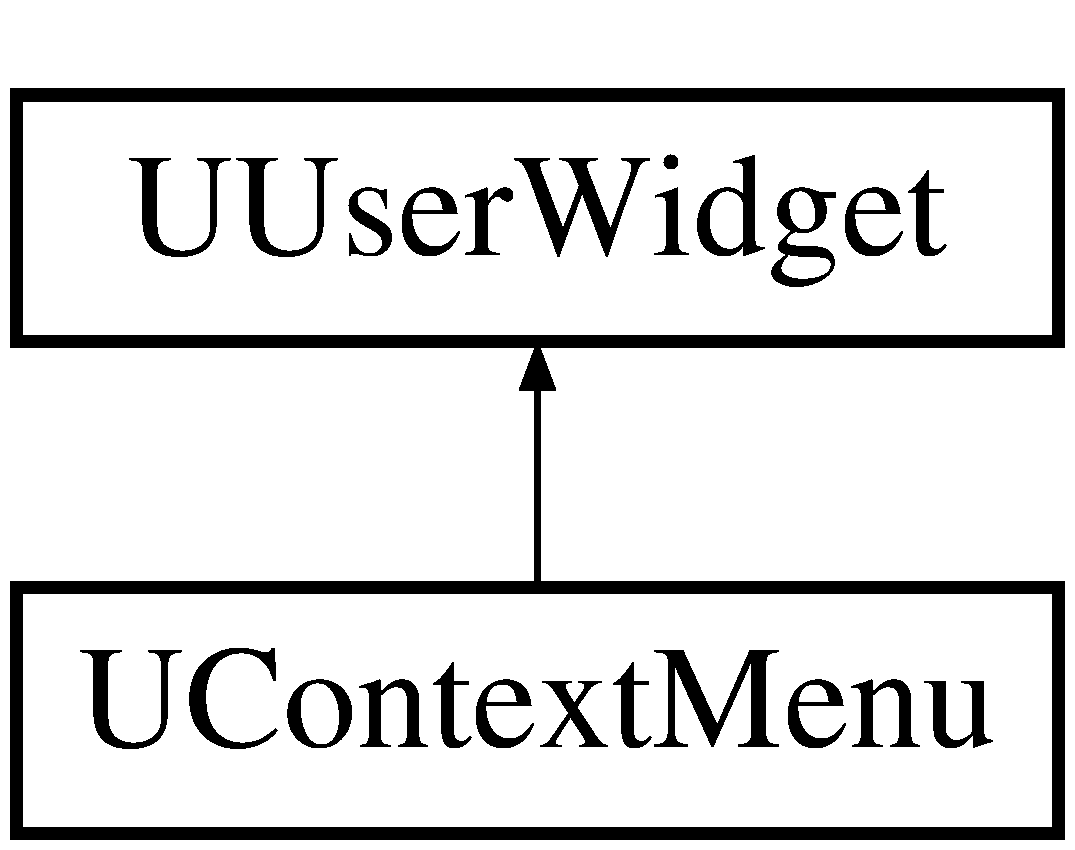
\includegraphics[height=2.000000cm]{class_u_context_menu}
\end{center}
\end{figure}
\subsection*{Public Attributes}
\begin{DoxyCompactItemize}
\item 
F\+String \hyperlink{class_u_context_menu_abed1c996540fc75dc7e495a6e56d6bfb}{Widget\+Name}
\begin{DoxyCompactList}\small\item\em A public variable. \end{DoxyCompactList}\end{DoxyCompactItemize}


\subsection{Detailed Description}
Class for UI. 

Contains necessary functions for the context menu in the gamescape. 

\subsection{Member Data Documentation}
\hypertarget{class_u_context_menu_abed1c996540fc75dc7e495a6e56d6bfb}{}\label{class_u_context_menu_abed1c996540fc75dc7e495a6e56d6bfb} 
\index{U\+Context\+Menu@{U\+Context\+Menu}!Widget\+Name@{Widget\+Name}}
\index{Widget\+Name@{Widget\+Name}!U\+Context\+Menu@{U\+Context\+Menu}}
\subsubsection{\texorpdfstring{Widget\+Name}{WidgetName}}
{\footnotesize\ttfamily F\+String U\+Context\+Menu\+::\+Widget\+Name}



A public variable. 

Name of the Widget 

The documentation for this class was generated from the following file\+:\begin{DoxyCompactItemize}
\item 
Context\+Menu.\+h\end{DoxyCompactItemize}

\hypertarget{class_x_a3}{}\section{X\+A3 Class Reference}
\label{class_x_a3}\index{X\+A3@{X\+A3}}
Inheritance diagram for X\+A3\+:\begin{figure}[H]
\begin{center}
\leavevmode
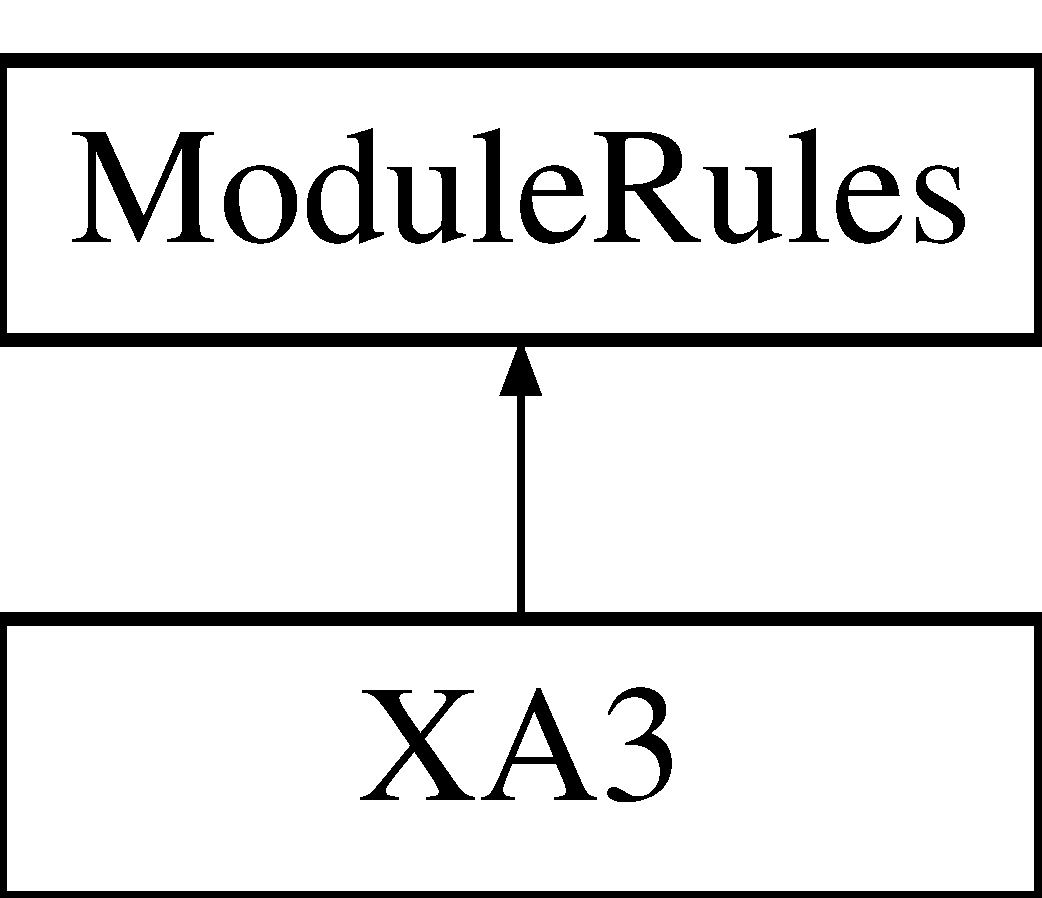
\includegraphics[height=2.000000cm]{class_x_a3}
\end{center}
\end{figure}
\subsection*{Public Member Functions}
\begin{DoxyCompactItemize}
\item 
\hypertarget{class_x_a3_a496c0d3cc1ba6008bc8ecd28d2e53f6f}{}\label{class_x_a3_a496c0d3cc1ba6008bc8ecd28d2e53f6f} 
{\bfseries X\+A3} (Target\+Info Target)
\end{DoxyCompactItemize}


The documentation for this class was generated from the following file\+:\begin{DoxyCompactItemize}
\item 
X\+A3.\+Build.\+cs\end{DoxyCompactItemize}

%--- End generated contents ---

% Index
\backmatter
\newpage
\phantomsection
\clearemptydoublepage
\addcontentsline{toc}{chapter}{Index}
\printindex

\end{document}
